\section{Durchführung und Auswertung}

\subsection{Sphärische Aberration}

Da sich die sphärische Aberration in allgemeiner Unschärfe des Bildes zeigt, wurde auf eine separate Abbildung verzichtet. Ihre Auswirkung ist jedoch auf den meisten Abbildungen zu erkennen; insbesondere äußert sie sich als Koma in Kombination mit dem Astigmatismus.

\subsection{Koma}

Zur Erzeugung der Koma wurde eine handelsübliche Linse mit einer Brennweite von $\SI{60}{\milli\meter}$ in schräger Befestigung verwendet. Das Objekt war ein Pinhole mit variablem Abstand zur optischen Achse. An den Abb. \ref{fig:koma_stark} und \ref{fig:koma_schwach} wird deutlich, dass die Koma mit dem Abstand zur optischen Achse zunimmt. 

Da die Koma als Kombination von sphärischer Aberration und Astigmatismus angesehen werden kann, kann sie durch Abblenden der Randstrahlen kompensiert werden. Dies wurde bei Abb. \ref{fig:koma_korrigiert} erreicht.

\begin{figure}[h!]
	\begin{minipage}[t]{0.32\textwidth}
		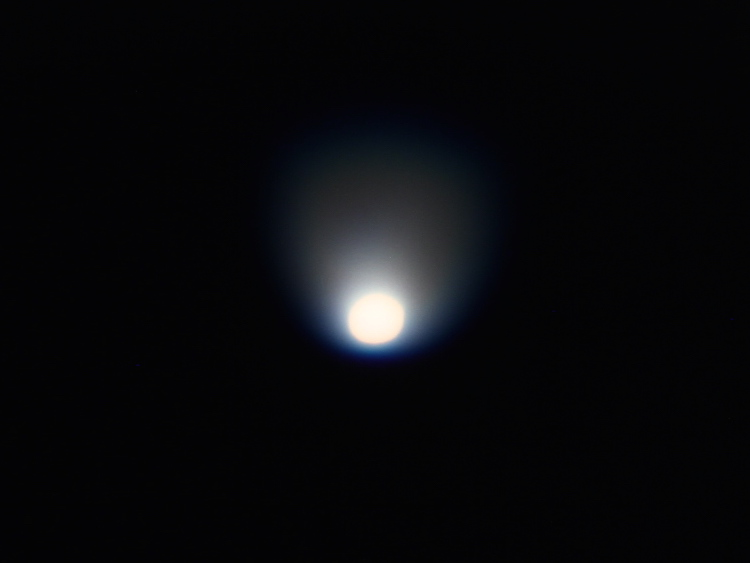
\includegraphics[width=\linewidth]{img/Koma/Prakt_Linsenfehler_2015_06_04_097}
		\caption{Starkes Koma am Außenrand der Linse}
		\label{fig:koma_stark}
	\end{minipage}
	\hfill
	\begin{minipage}[t]{0.32\textwidth}
		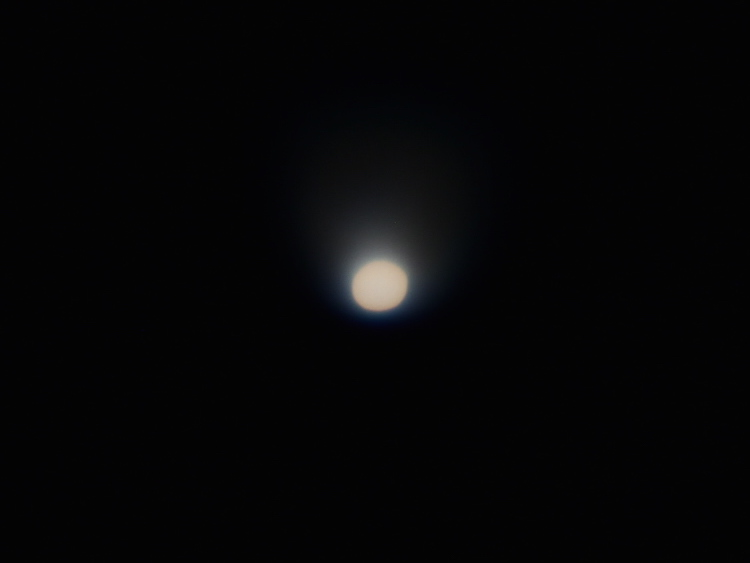
\includegraphics[width=\linewidth]{img/Koma/Prakt_Linsenfehler_2015_06_04_096}
		\caption{Schwaches Koma nahe der optischen Achse}
		\label{fig:koma_schwach}
	\end{minipage}
	\hfill
	\begin{minipage}[t]{0.32\textwidth}
		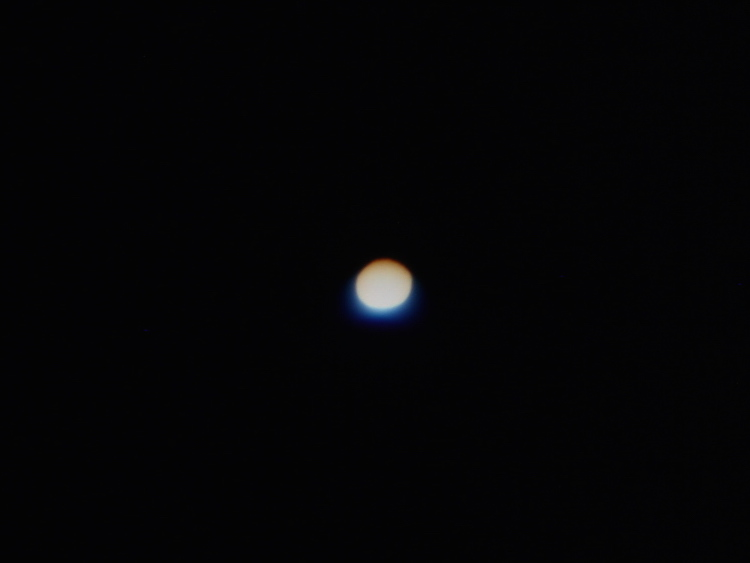
\includegraphics[width=\linewidth]{img/Koma/Prakt_Linsenfehler_2015_06_04_099}
		\caption{Abbildung mit Korrektur der Koma}
		\label{fig:koma_korrigiert}
	\end{minipage}	
\end{figure}

\subsection{Astigmatismus}

Der Nachweis des Astigmatismus erfolgte durch eine Linse, die sowohl gerade achsennormal (Abb. \ref{fig:astigmatismus_0}) als auch schräg zur optischen Achse (Abb. \ref{fig:astigmatismus_meridional} bis \ref{fig:astigmatismus_mittenfokus}) befestigt wurde. Als Objekt diente ein Pinhole auf der optischen Achse. 

Durch den so erreichten schrägen Einfall der Strahlenbündel werden diese abhängig von ihrer Zugehörigkeit zur Meridional- bzw. Sagittalebene in unterschiedlichen Brennweiten fokussiert, die separat abgebildet werden können. Bei Platzierung der Bildebene zwischen den Brennweiten ergibt sich eine Superposition der Einzelbrennpunkte (Abb. \ref{fig:astigmatismus_mittenfokus}).

\begin{figure}[h!]
	\begin{minipage}[t]{0.48\textwidth}
		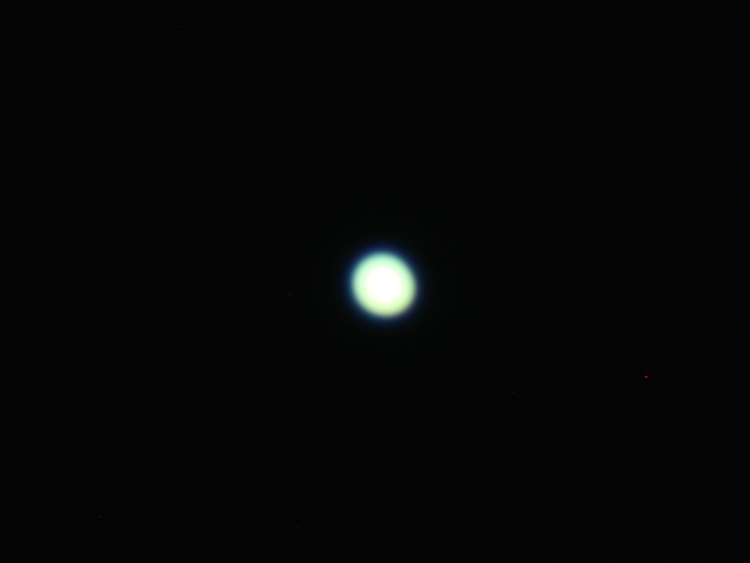
\includegraphics[width=\linewidth]{img/Astigmatismus/Prakt_Linsenfehler_2015_06_04_086}
		\caption{Abbildung ohne Astigmatismus}
		\label{fig:astigmatismus_0}
	\end{minipage}
	\hfill
	\begin{minipage}[t]{0.48\textwidth}
		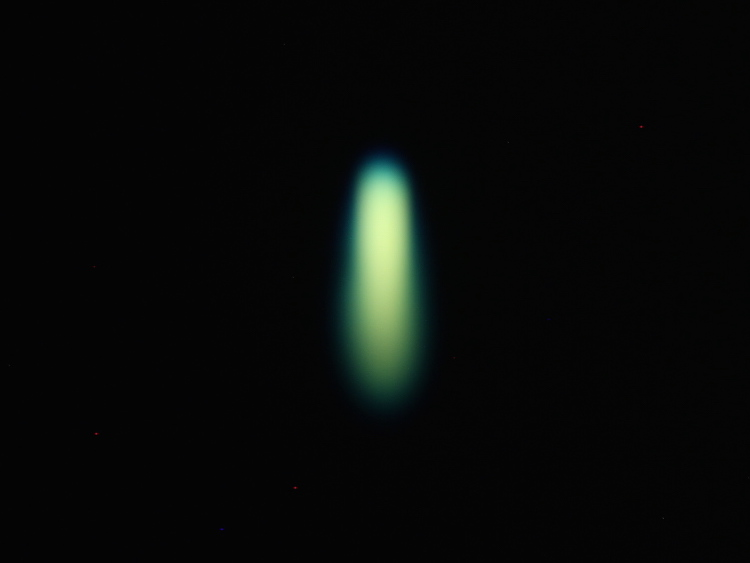
\includegraphics[width=\linewidth]{img/Astigmatismus/Prakt_Linsenfehler_2015_06_04_088_meridional}
		\caption{Abbildung der Meridionalebene}
		\label{fig:astigmatismus_meridional}
	\end{minipage}
	
	\vspace{0.5cm}
	
	\begin{minipage}[t]{0.48\textwidth}
		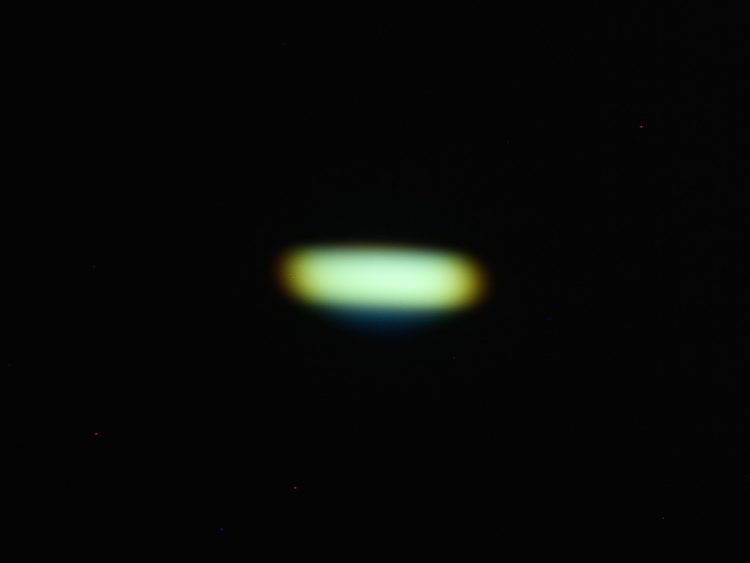
\includegraphics[width=\linewidth]{img/Astigmatismus/Prakt_Linsenfehler_2015_06_04_087_saggital}
		\caption{Abbildung der Sagitalebene}
		\label{fig:astigmatismus_sagittal}
	\end{minipage}
	\hfill
	\begin{minipage}[t]{0.48\textwidth}
		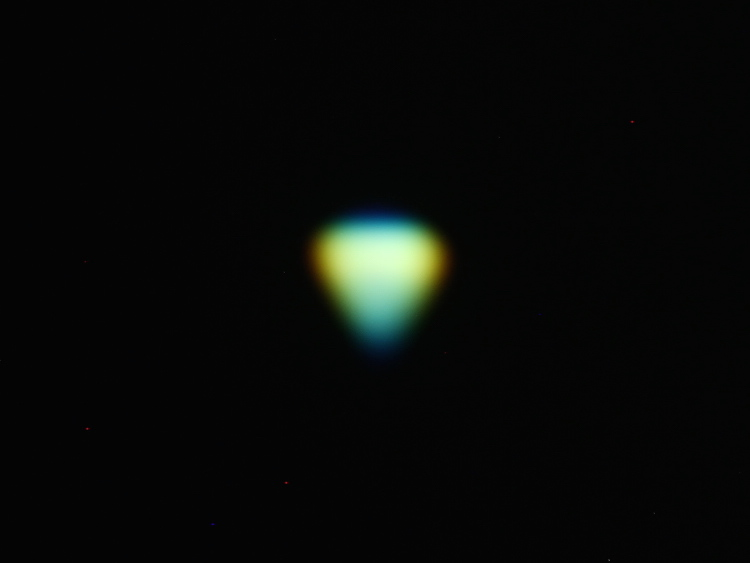
\includegraphics[width=\linewidth]{img/Astigmatismus/Prakt_Linsenfehler_2015_06_04_089_mittenfokus}
		\caption{Fokus zwischen meridionaler und sagittaler Abbildung}
		\label{fig:astigmatismus_mittenfokus}
	\end{minipage}
\end{figure}

\subsection{Bildfeldwölbung}

Um die Bildfeldwölbung zu veranschaulichen, wurde ein Raster durch einen $\SI{60}{\milli\meter}$-Achromaten abgebildet. Anhand des in Abb. \ref{fig:bildwoelbung_aussen} und \ref{fig:bildwoelbung_mitte} verwendeten planaren Schirms wird deutlich, dass die Schärfebereiche jeweils konzentrische Kreise sind, da die fokussierte Abbildung auf einer Kugeloberfläche erfolgt (die Schnittkurve von Kugel und Ebene ist ein Kreis). 

In Abb. \ref{fig:bildwoelbung_korrigiert} wurde manuell eine Korrekturmöglichkeit in Form eines vertikal gekrümmten Schirms (Zylindermantelfläche) nachgebildet. Es ist zu erkennen, dass das Bild dadurch in vertikaler Richtung scharf bleibt, in horizontaler jedoch nicht.

\begin{figure}[h!]
	\begin{minipage}[t]{0.48\textwidth}
		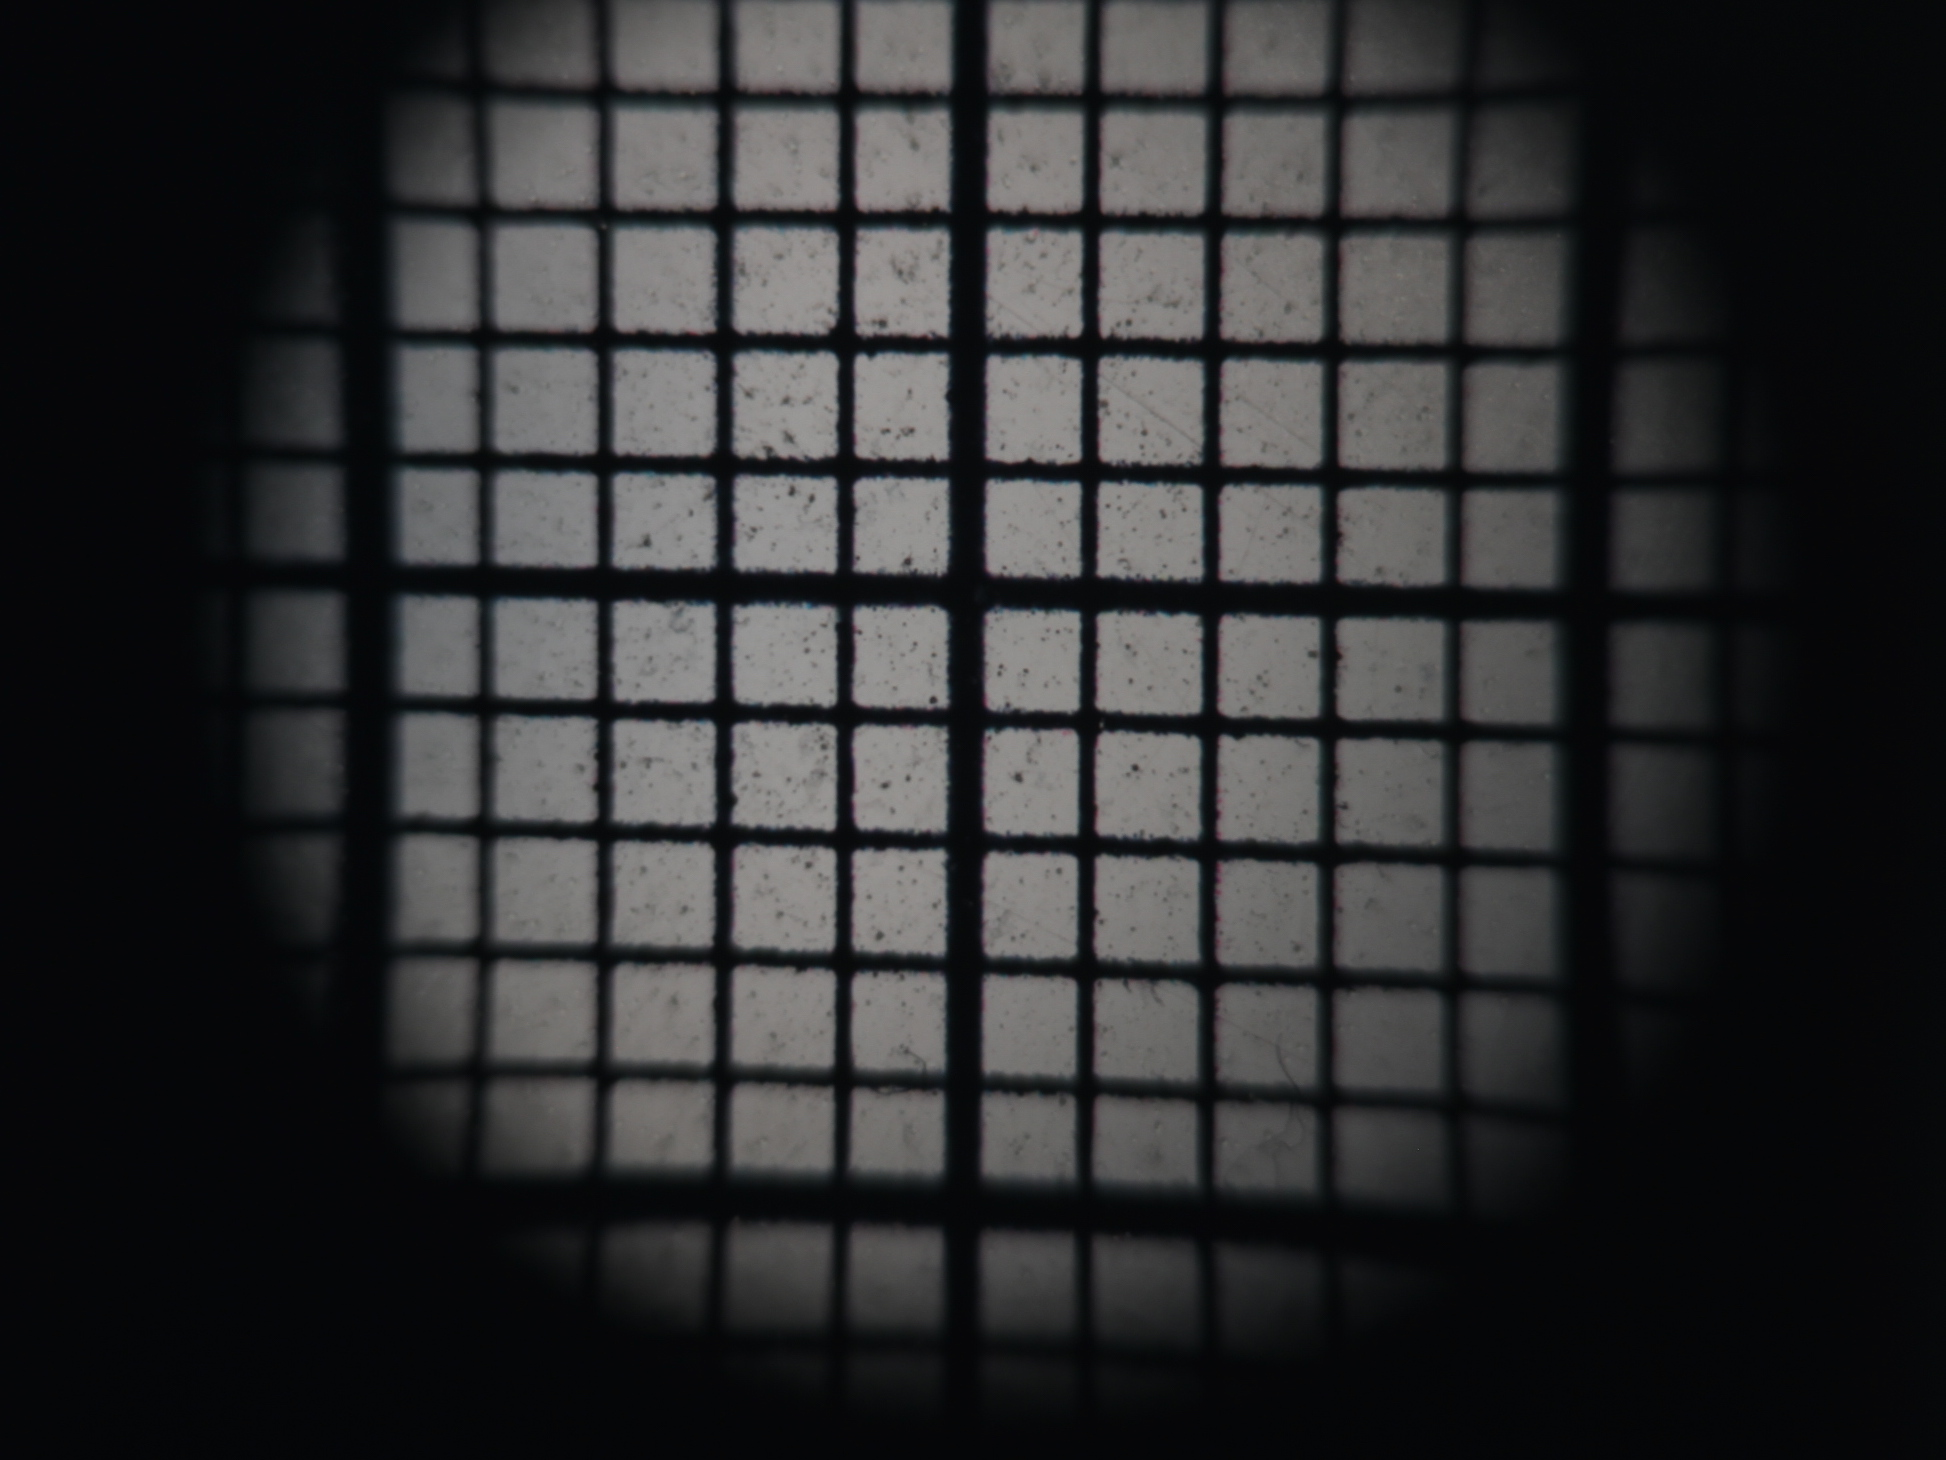
\includegraphics[width=\linewidth]{img/Bildwoelbung/Prakt_Linsenfehler_2015_06_04_074}
		\caption{Unschärfe am Außenrand des Gitters}
		\label{fig:bildwoelbung_aussen}
	\end{minipage}
	\hfill
	\begin{minipage}[t]{0.48\textwidth}
		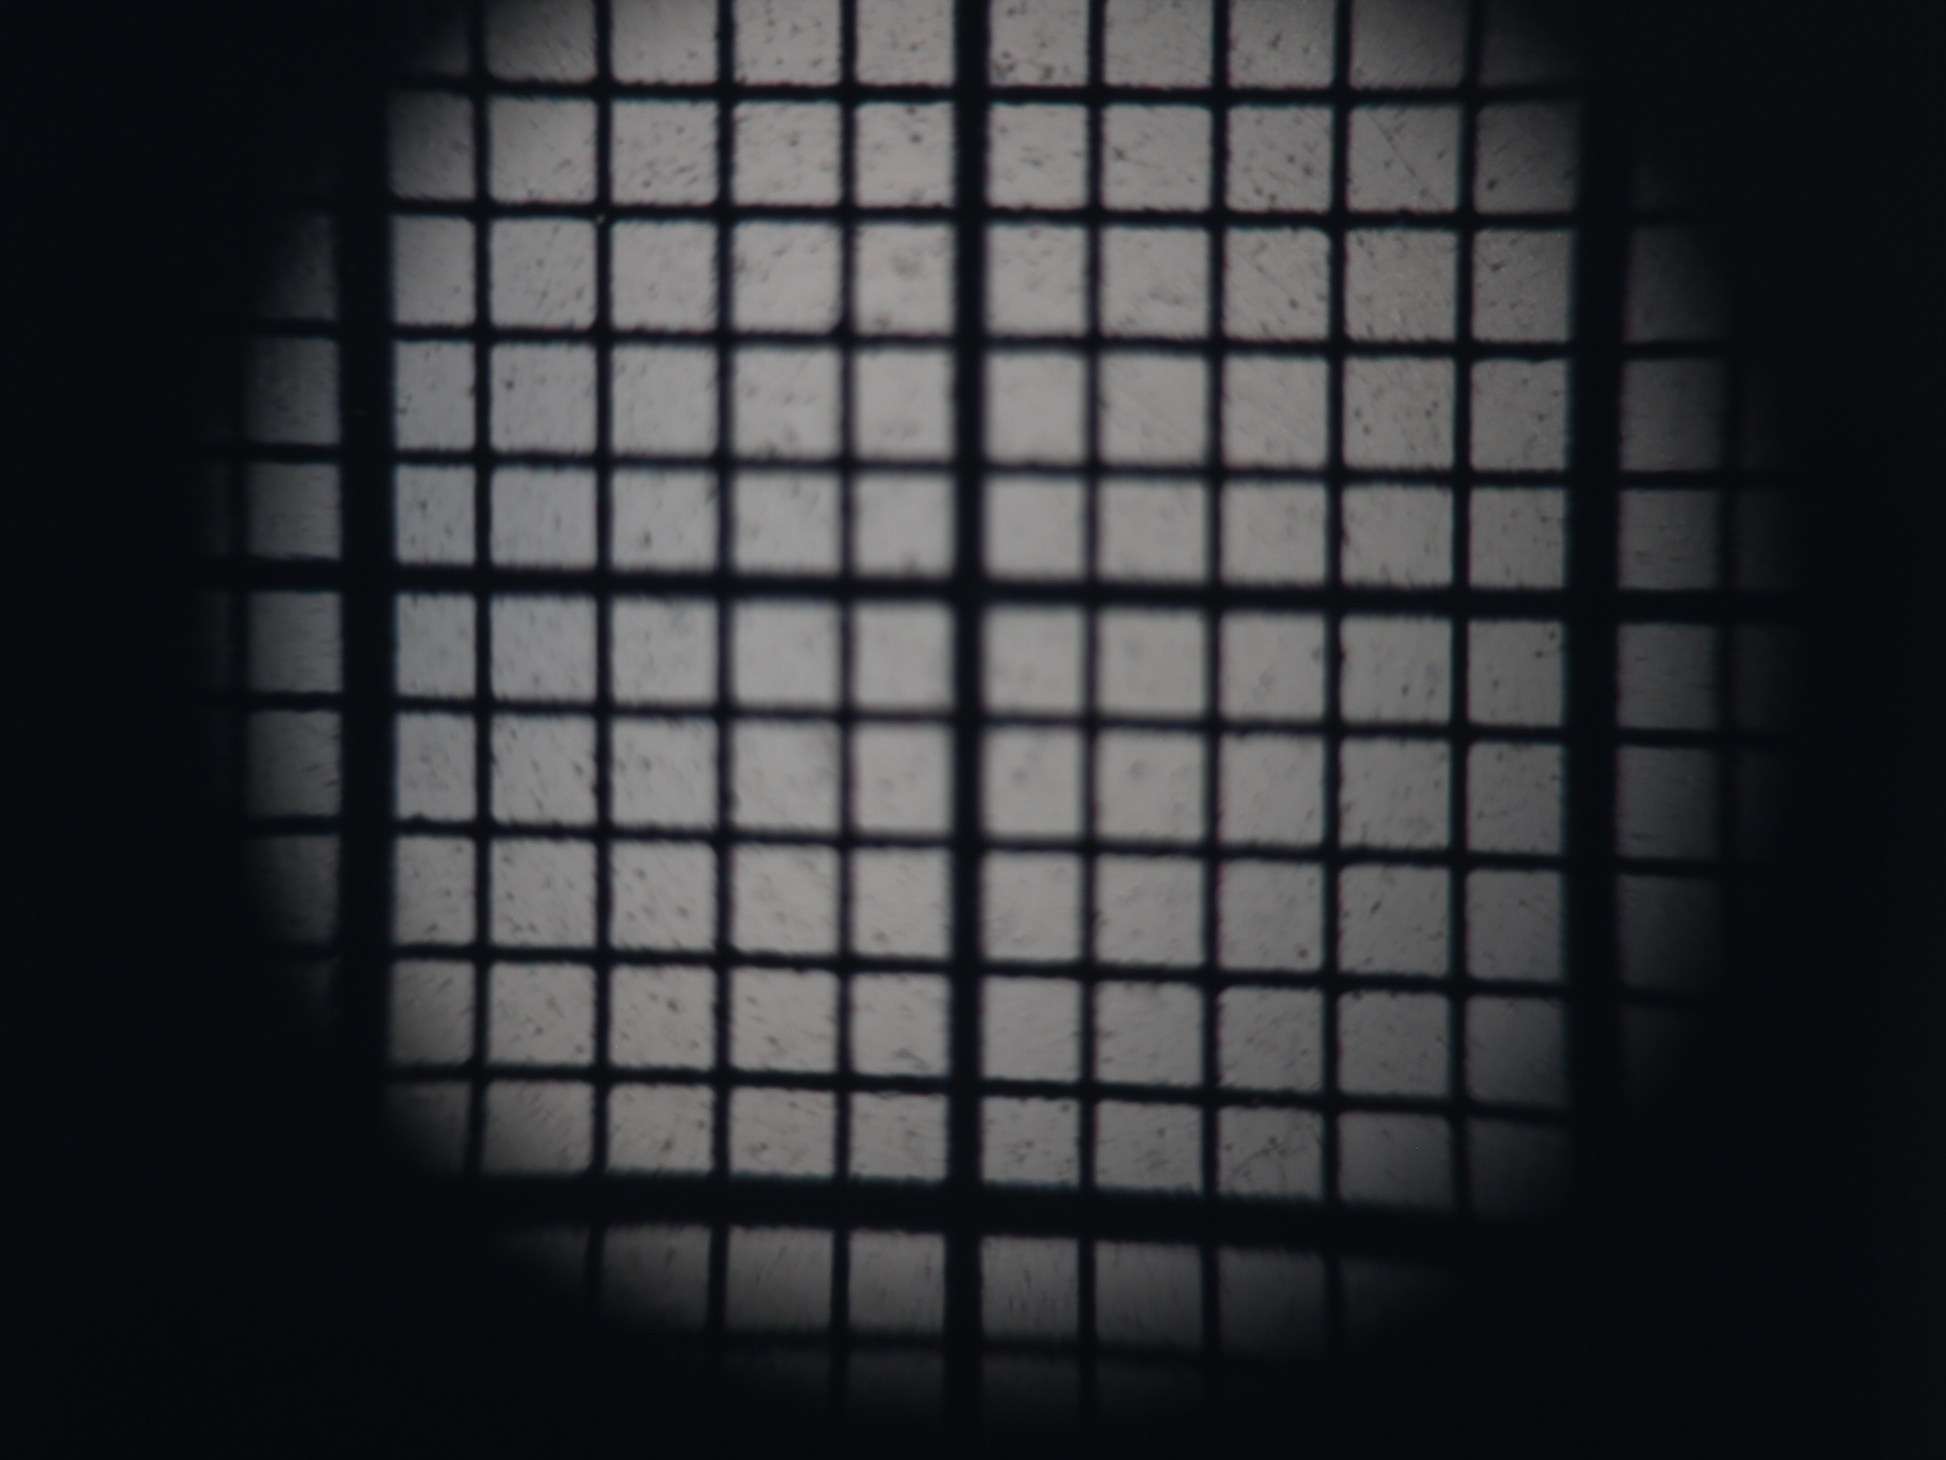
\includegraphics[width=\linewidth]{img/Bildwoelbung/Prakt_Linsenfehler_2015_06_04_075}
		\caption{Unschärfe in der Mitte des Gitters}
		\label{fig:bildwoelbung_mitte}
	\end{minipage}
\end{figure}

\begin{figure}[h!]
	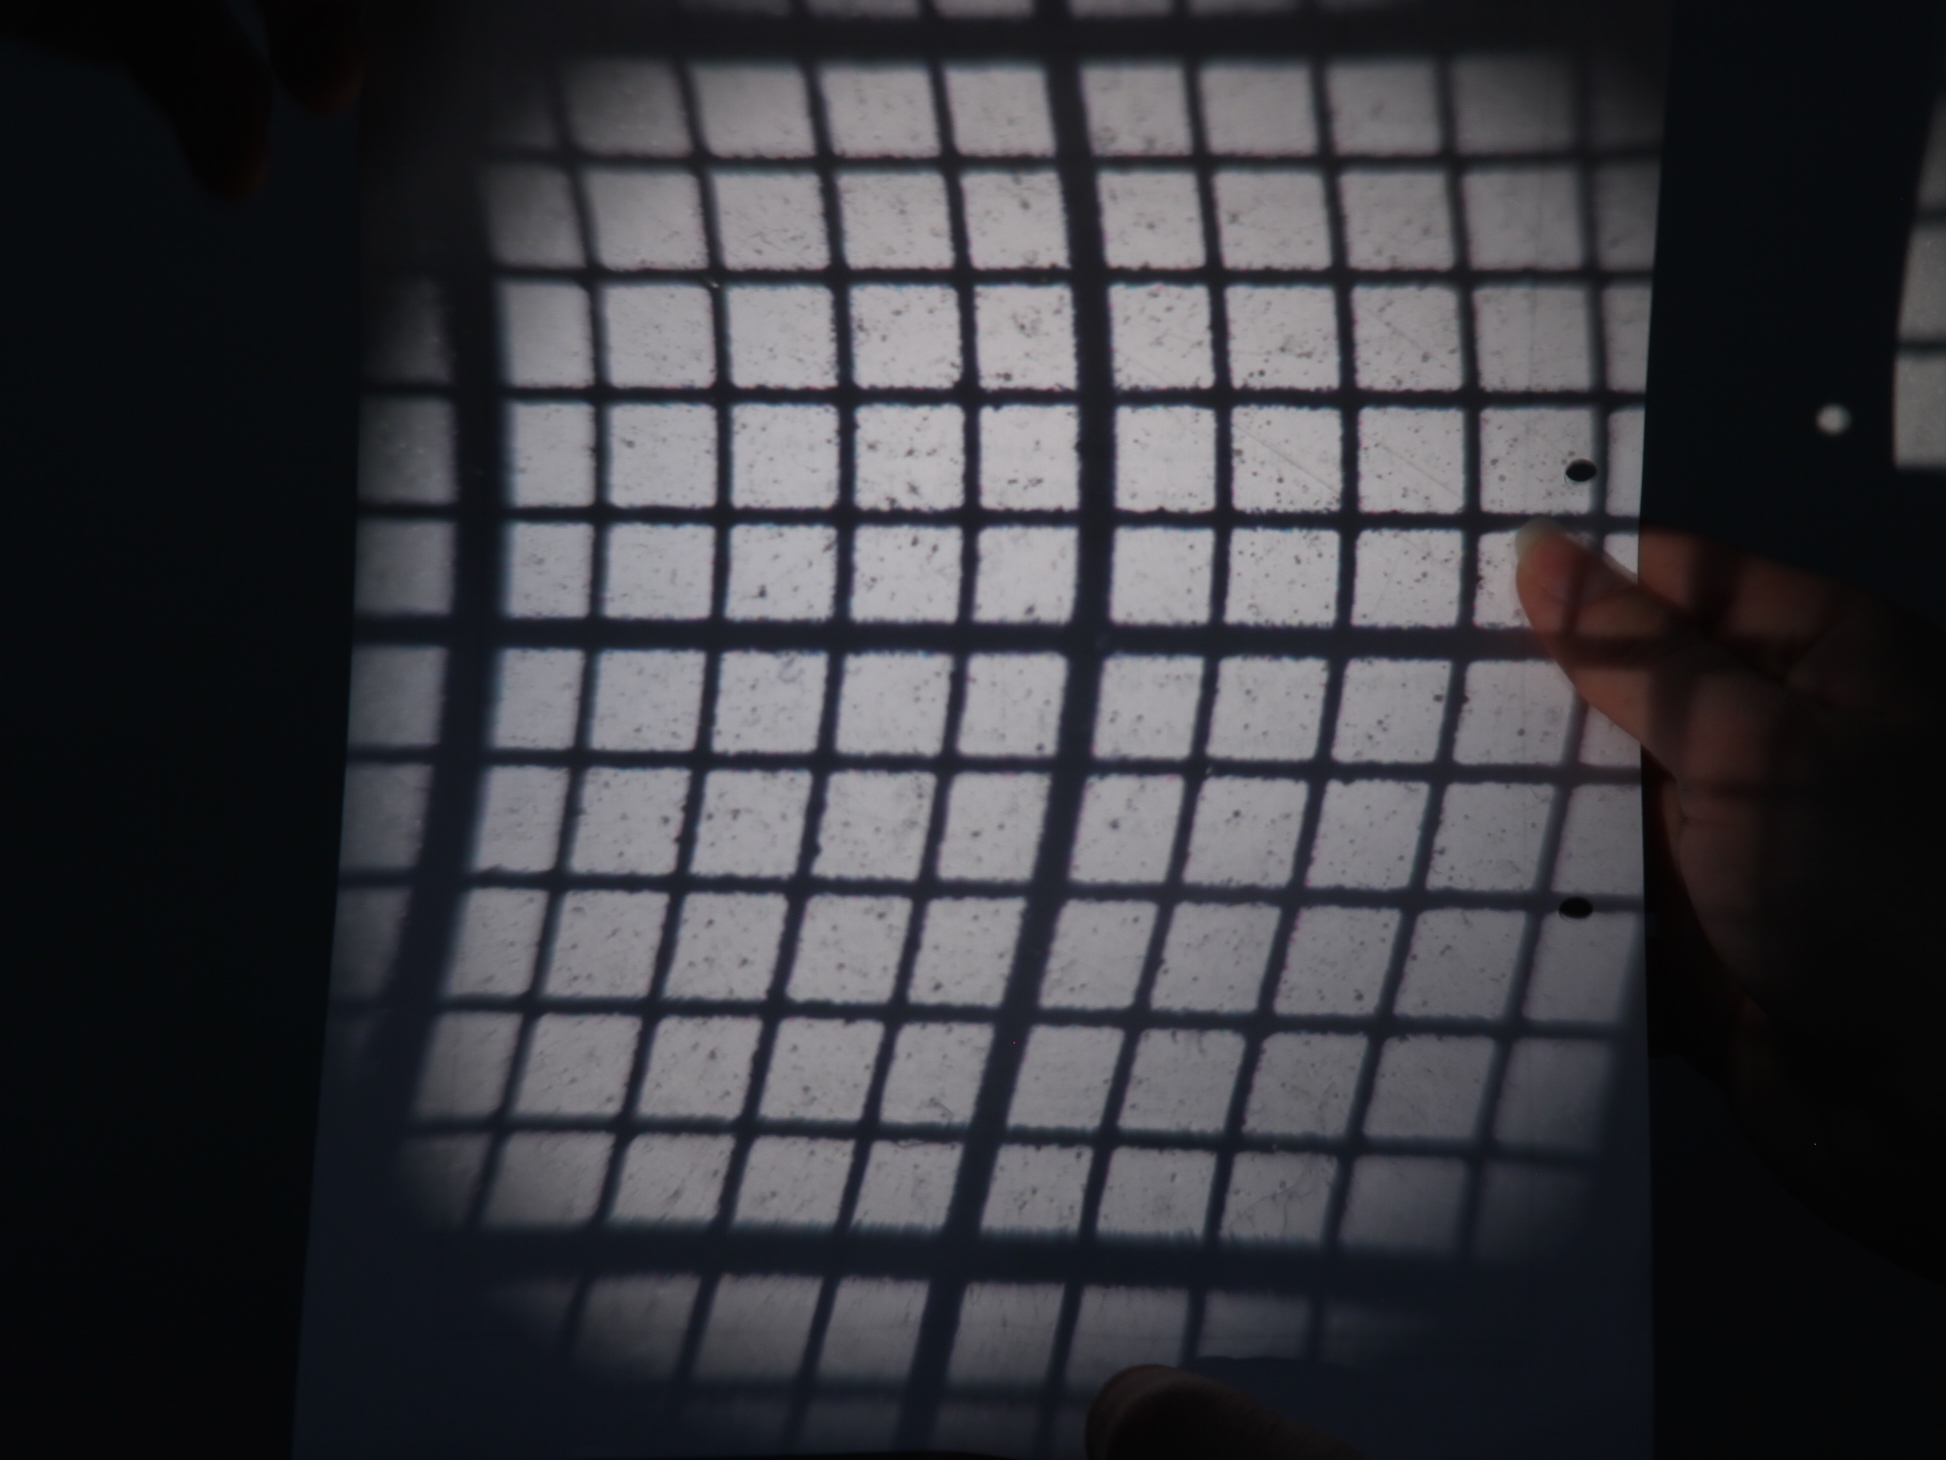
\includegraphics[width=\linewidth]{img/Bildwoelbung/Prakt_Linsenfehler_2015_06_04_076}
	\caption{Korrektur der Bildfeldwölbung durch gekrümmten Projektionsschirm}
	\label{fig:bildwoelbung_korrigiert}
\end{figure}

\subsection{Verzeichnung}

\begin{figure}[h!]
	\begin{minipage}[t]{0.48\textwidth}
		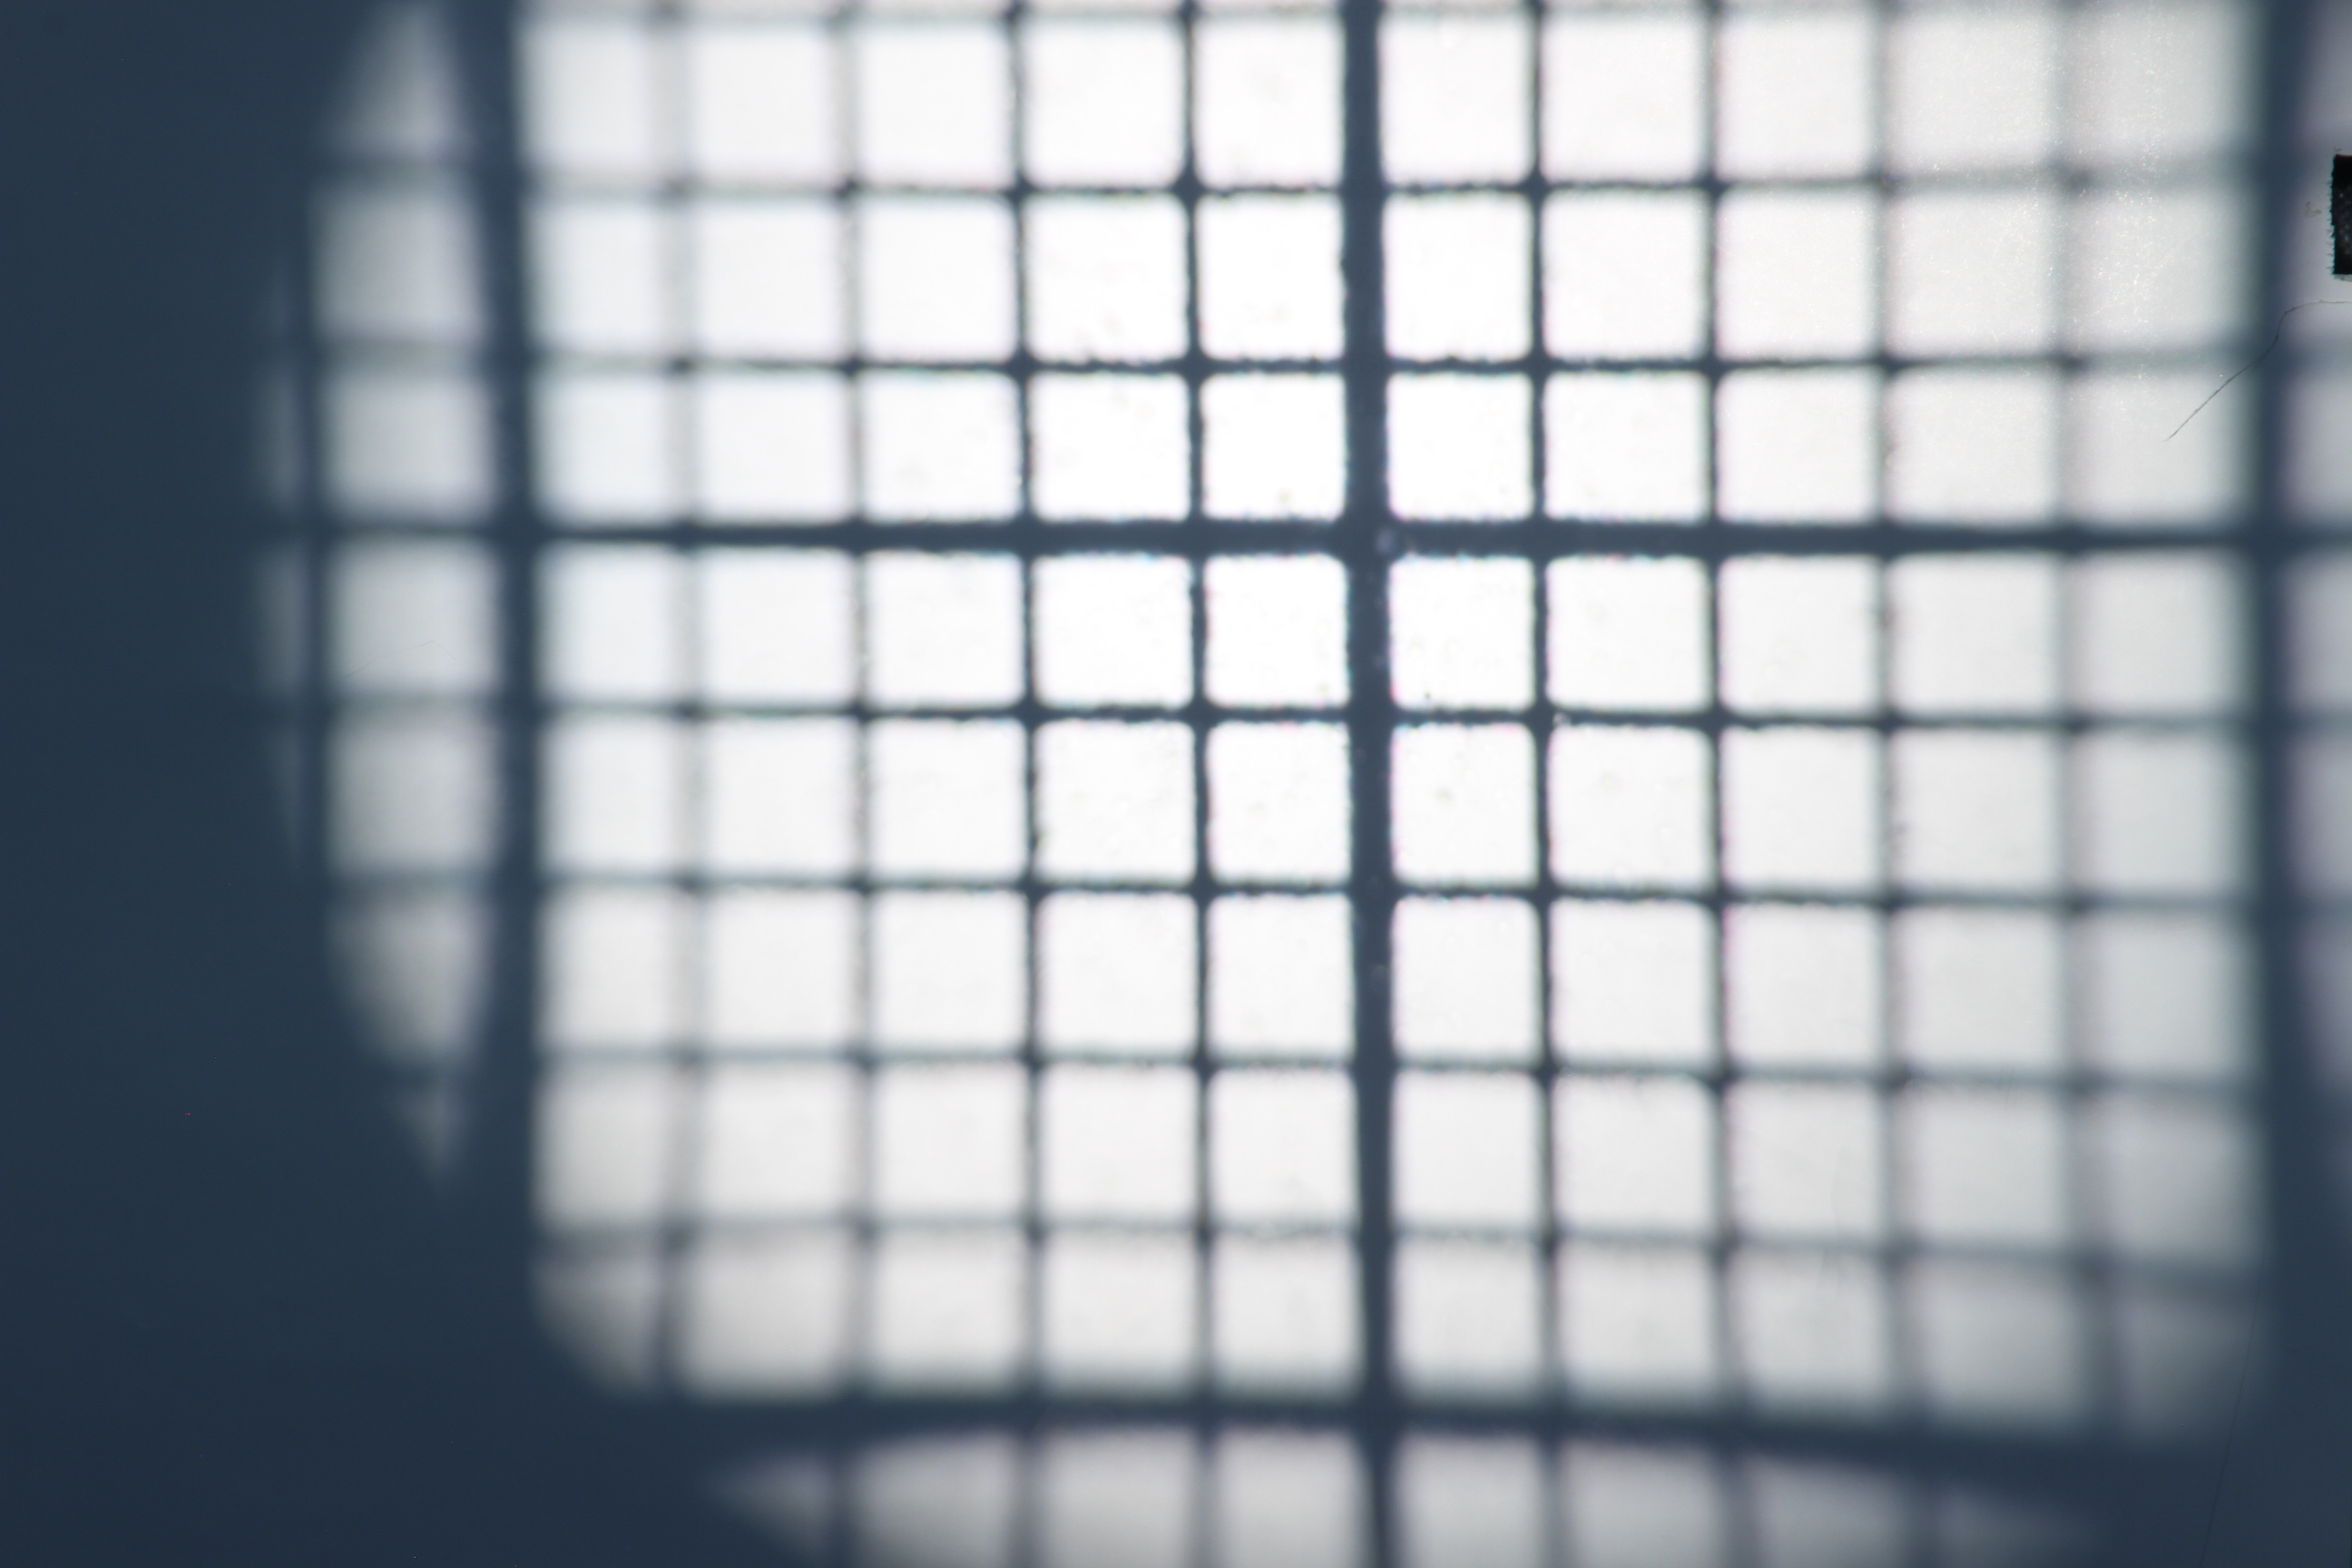
\includegraphics[width=\linewidth]{img/Verzeichnung/Prakt_Linsenfehler_2015_06_04_082}
		\caption{Am Rand des Gitters erkennbare Krümmung}
		\label{fig:verzeichnung}
	\end{minipage}
	\hfill
	\begin{minipage}[t]{0.48\textwidth}
		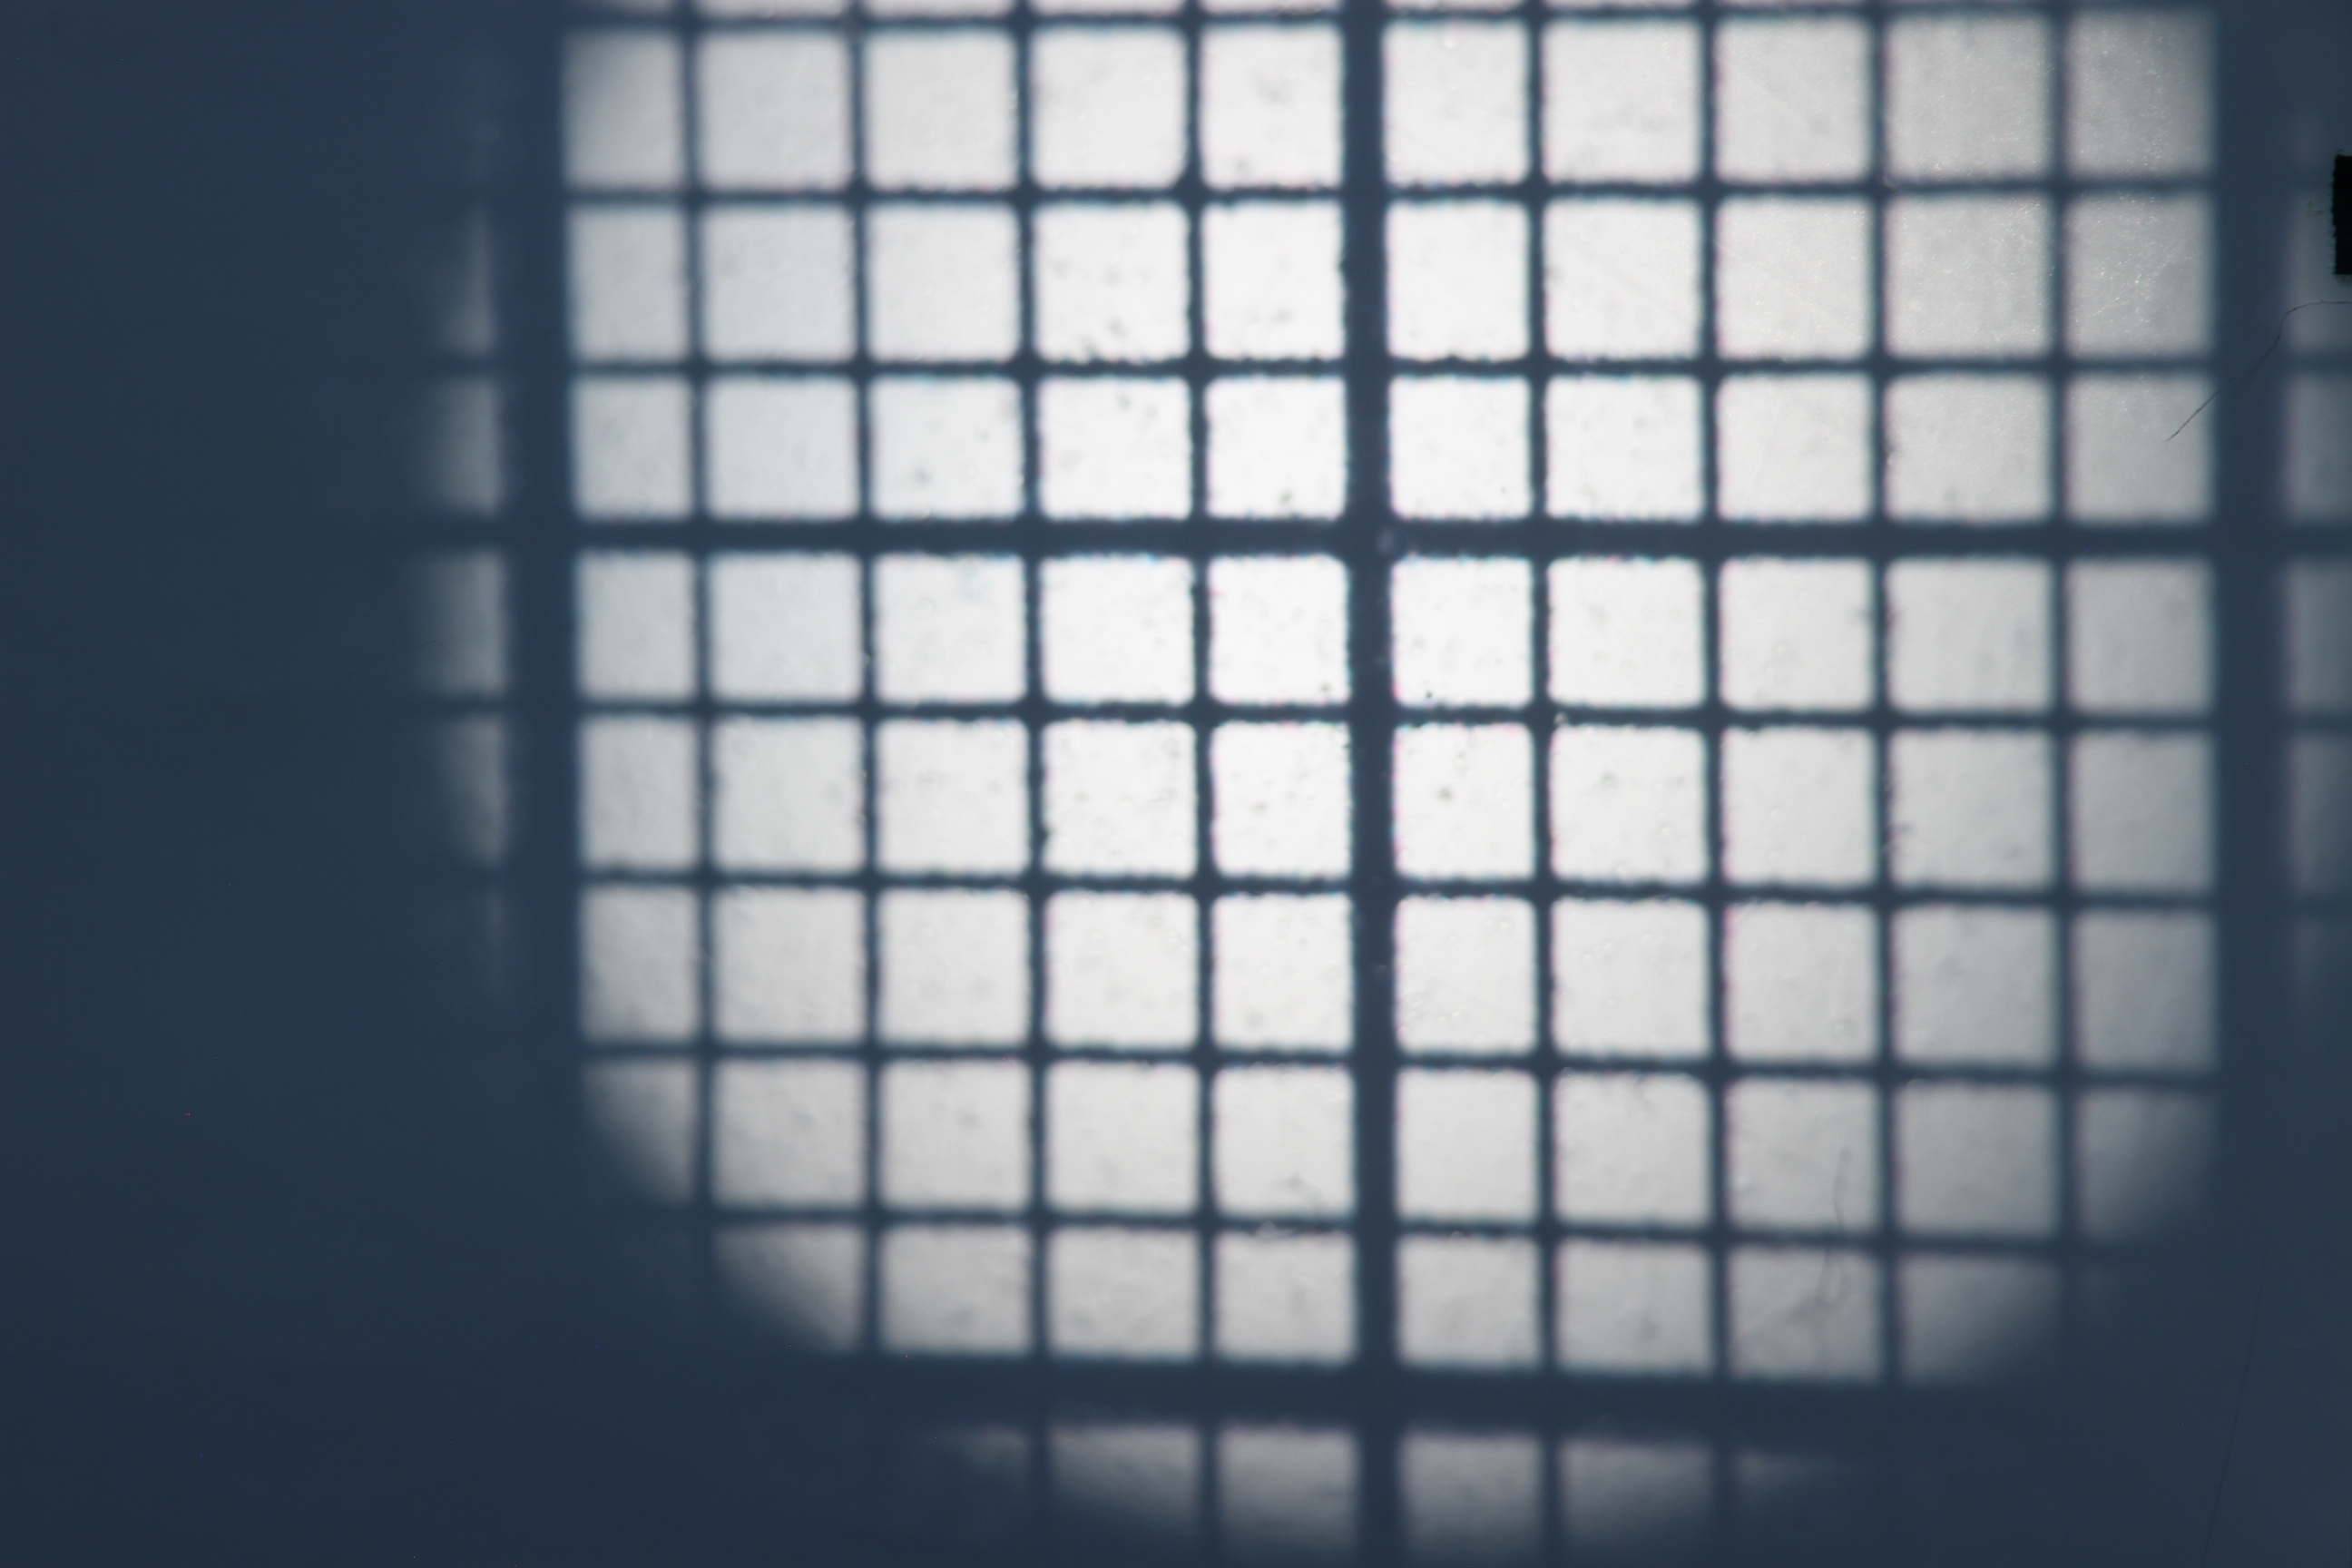
\includegraphics[width=\linewidth]{img/Verzeichnung/Prakt_Linsenfehler_2015_06_04_083}
		\caption{Korrektur der Verzeichnung}
		\label{fig:verzeichnung_korrigiert}
	\end{minipage}
\end{figure}

\subsection{Chromatische Aberration}

Zur Demonstration der chromatischen Aberration wurden eine gewöhnliche $\SI{60}{\milli\meter}$-Linse und ein Achromat gleicher Brennweite eingesetzt. Als Objekt diente wiederum das Raster. Mittels eines Farbfilters wurden jeweils die kurzwelligeren Strahlen der blauen Anteile fokussiert. Anschließend folgte durch Umschalten des Farbfilters bei unveränderter Anordnung der optischen Elemente ein Vergleich mit den Strahlen des grünen bzw. roten Lichts.

Es ist, insbesondere an der Verschmutzung des Rasters, zu erkennen, dass bei Verwendung der gewöhnlichen Linse die Schärfe mit zunehmender spektraler Entfernung der fokussierten Wellenlänge abnimmt (Abb. \ref{fig:cm_blau} bis \ref{fig:cm_rot}). Das rote Licht ist gegenüber dem blauen deutlich defokussiert. Beim Achromaten ist das nicht der Fall (Abb. \ref{fig:cm_blau_achromat} bis \ref{fig:cm_rot_achromat}).

\begin{figure}[h!]
	\begin{minipage}[t]{0.32\textwidth}
		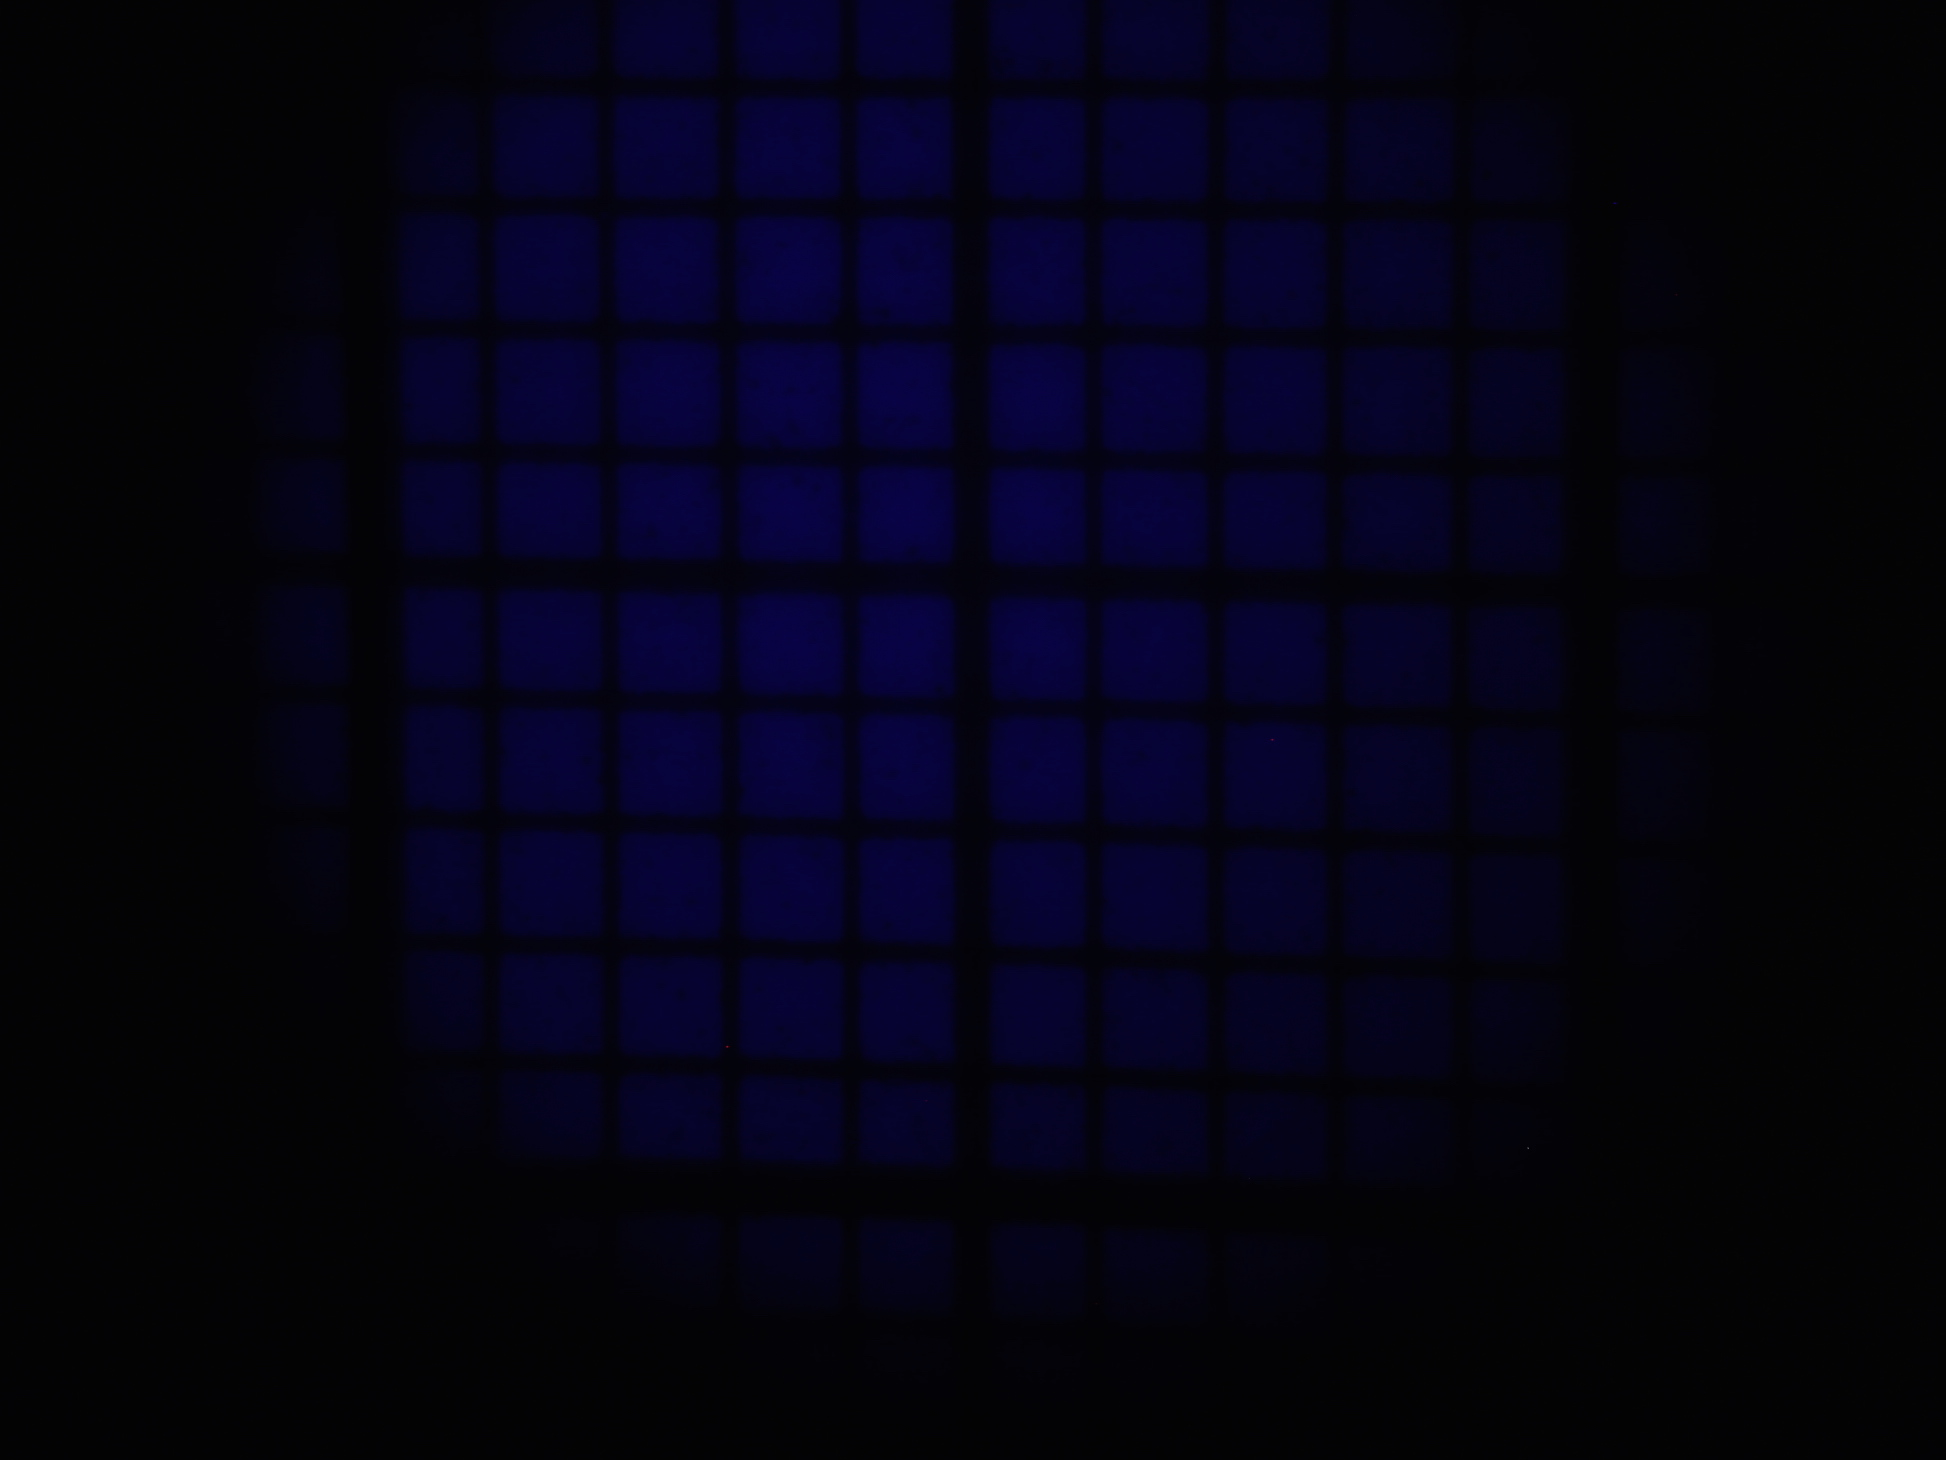
\includegraphics[clip=true, trim=700px 950px 900px 250px, width=\linewidth]{img/ChromAbb/Prakt_Linsenfehler_2015_06_04_068}
		\caption{Fokussierte Abbildung der blauen Wellenlängen (gewöhnliche Linse)}
		\label{fig:cm_blau}
	\end{minipage}
	\hfill
	\begin{minipage}[t]{0.32\textwidth}
		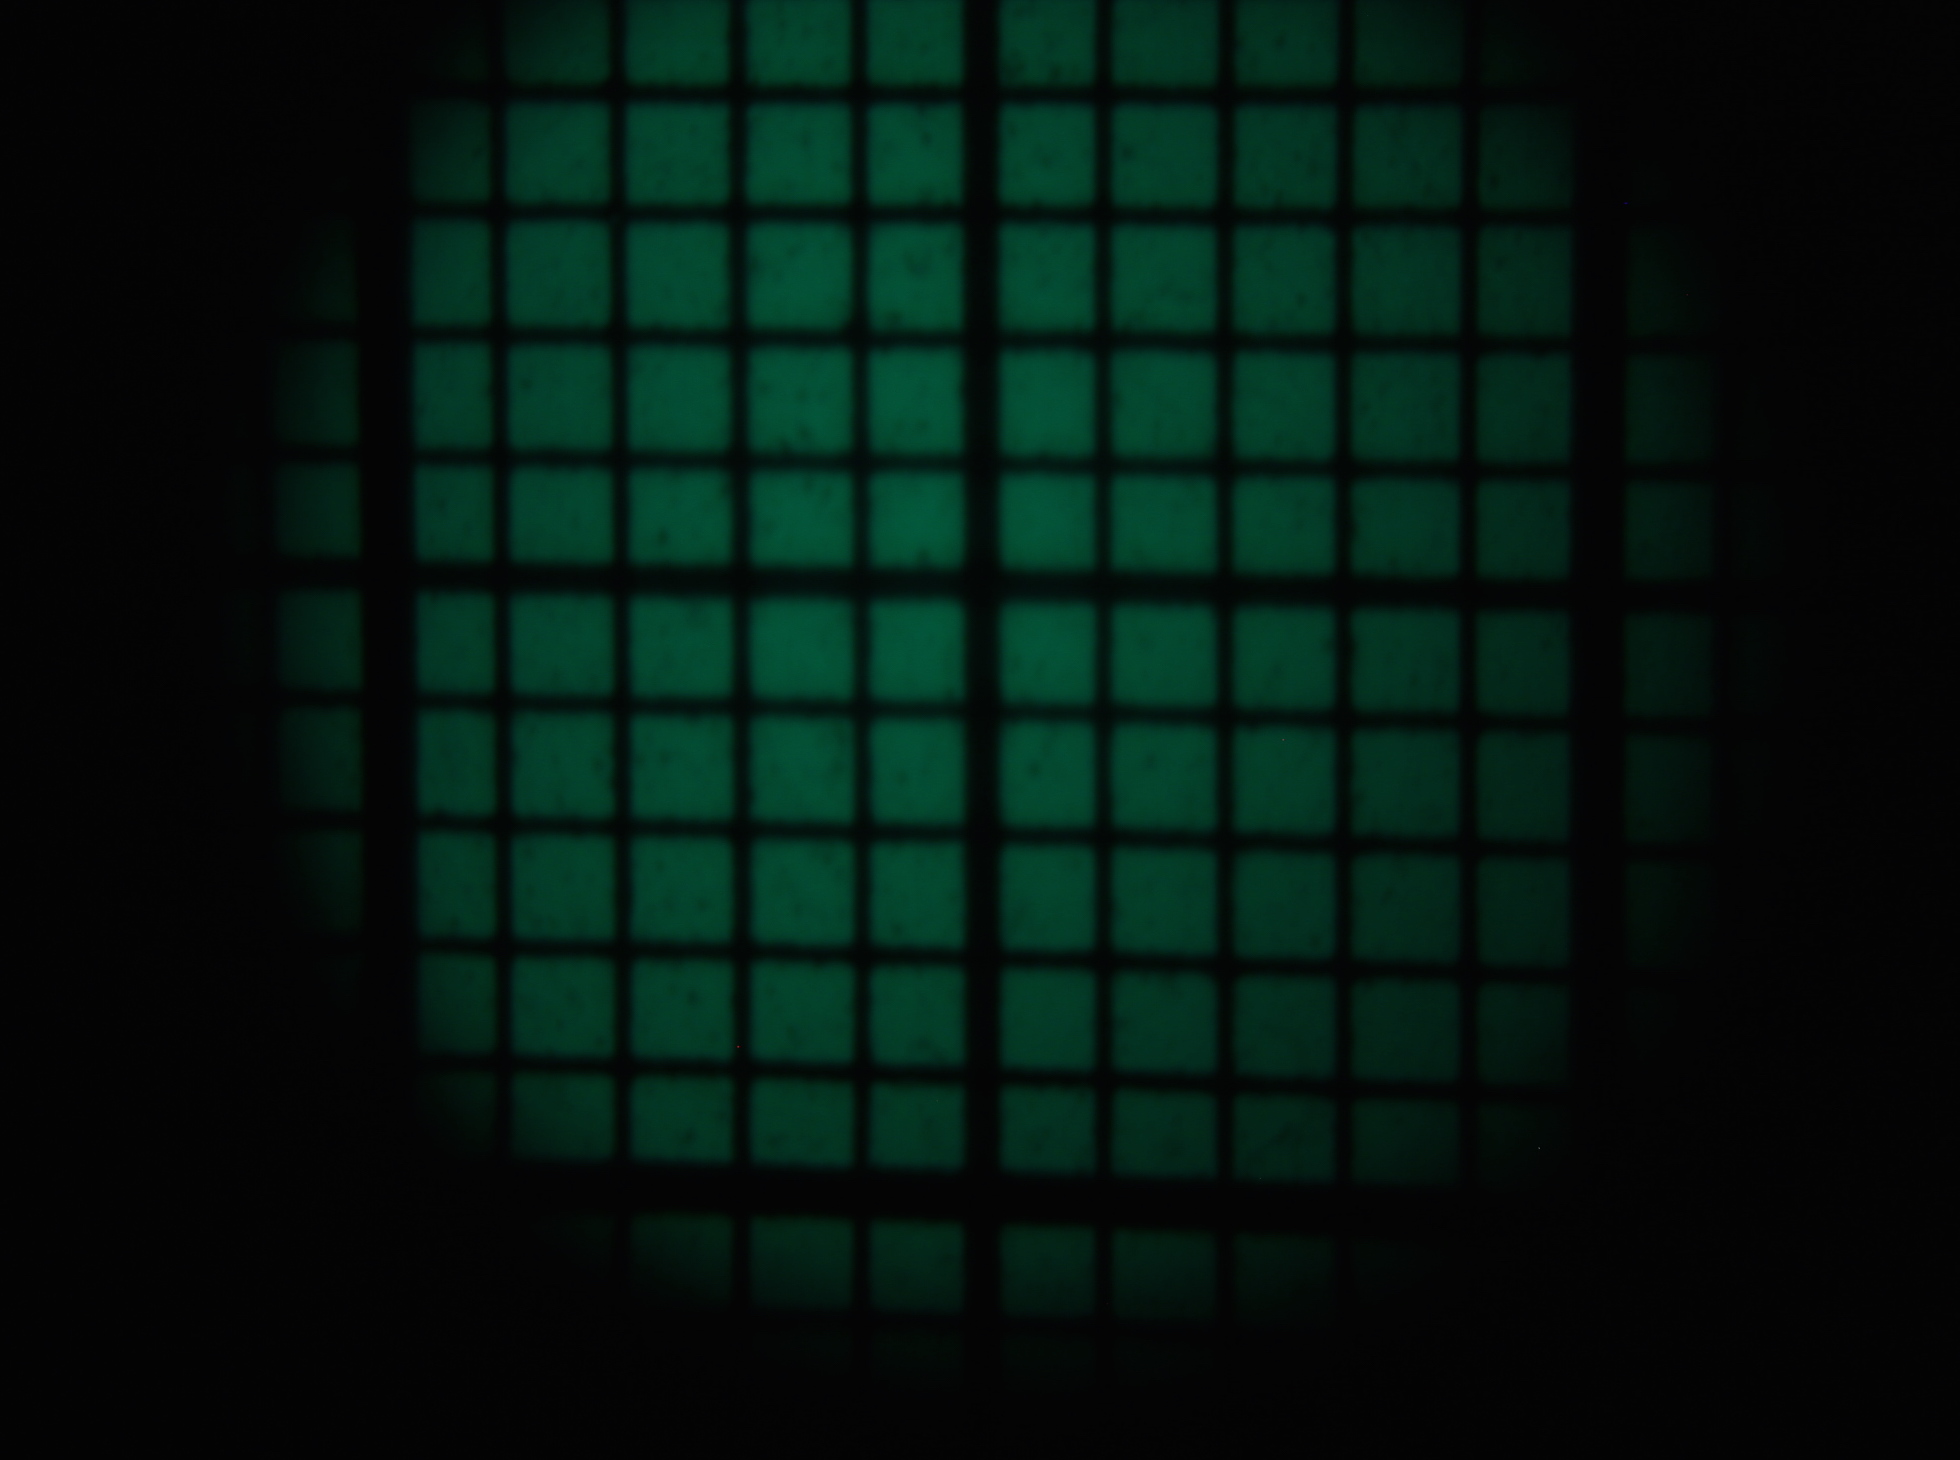
\includegraphics[clip=true, trim=707px 950px 907px 250px, width=\linewidth]{img/ChromAbb/Prakt_Linsenfehler_2015_06_04_069}
		\caption{Leicht defokussierte Abbildung der grünen Wellenlängen (gewöhnliche Linse)}
		\label{fig:cm_gruen}
	\end{minipage}
	\hfill
	\begin{minipage}[t]{0.32\textwidth}
		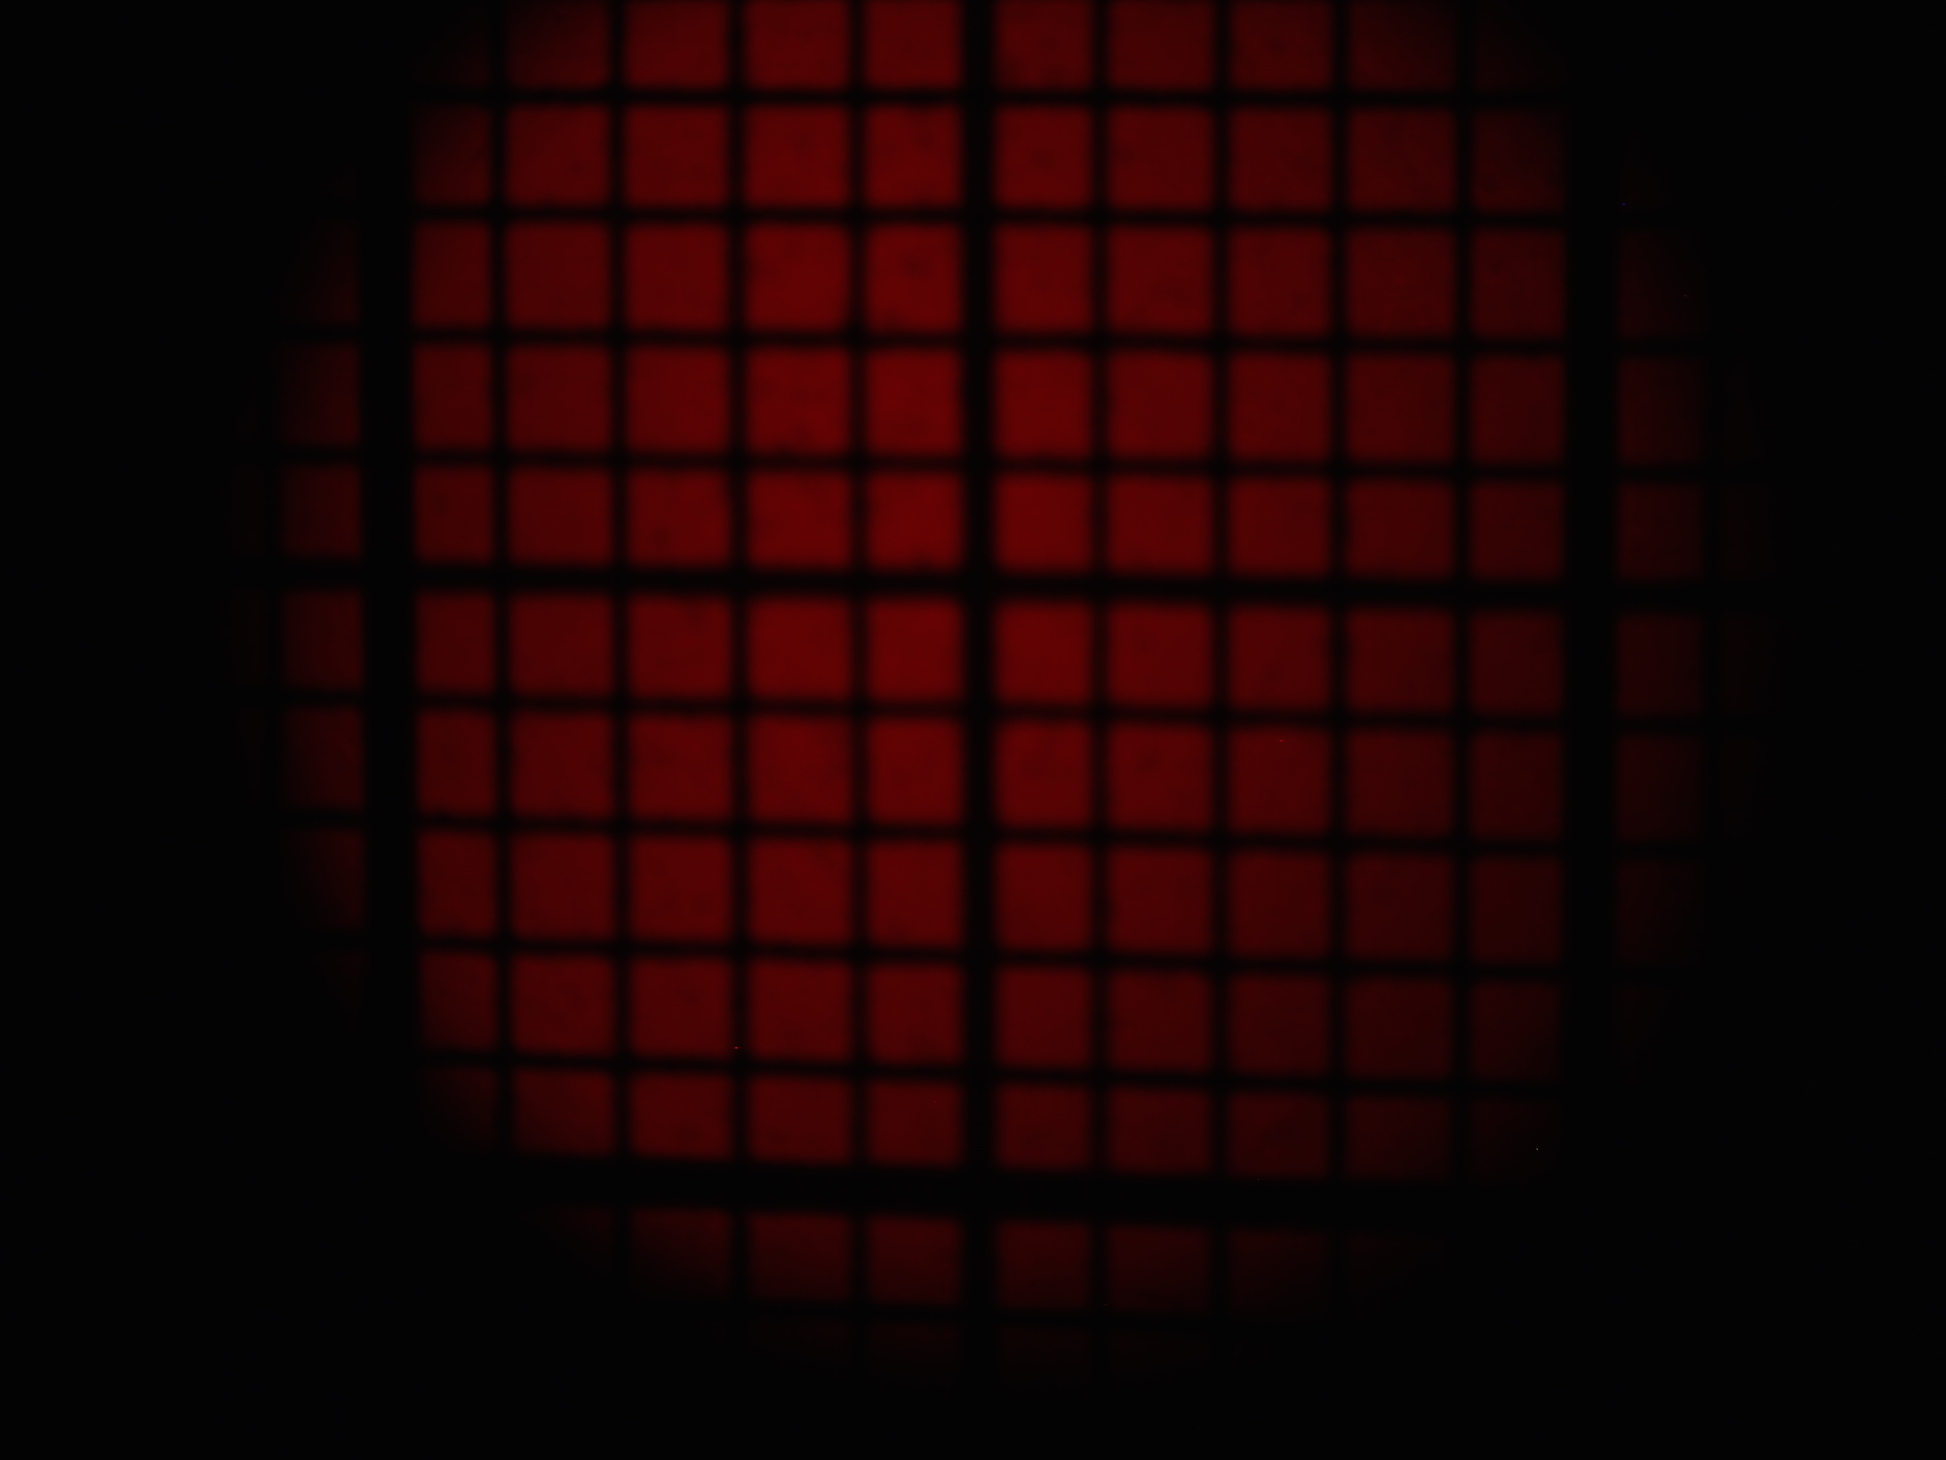
\includegraphics[clip=true, trim=700px 950px 900px 250px, width=\linewidth]{img/ChromAbb/Prakt_Linsenfehler_2015_06_04_070}
		\caption{Defokussierte Abbildung der roten Wellenlängen (gewöhnliche Linse)}
		\label{fig:cm_rot}
	\end{minipage}
		
	\vspace{0.5cm}
	
	\begin{minipage}[t]{0.32\textwidth}
		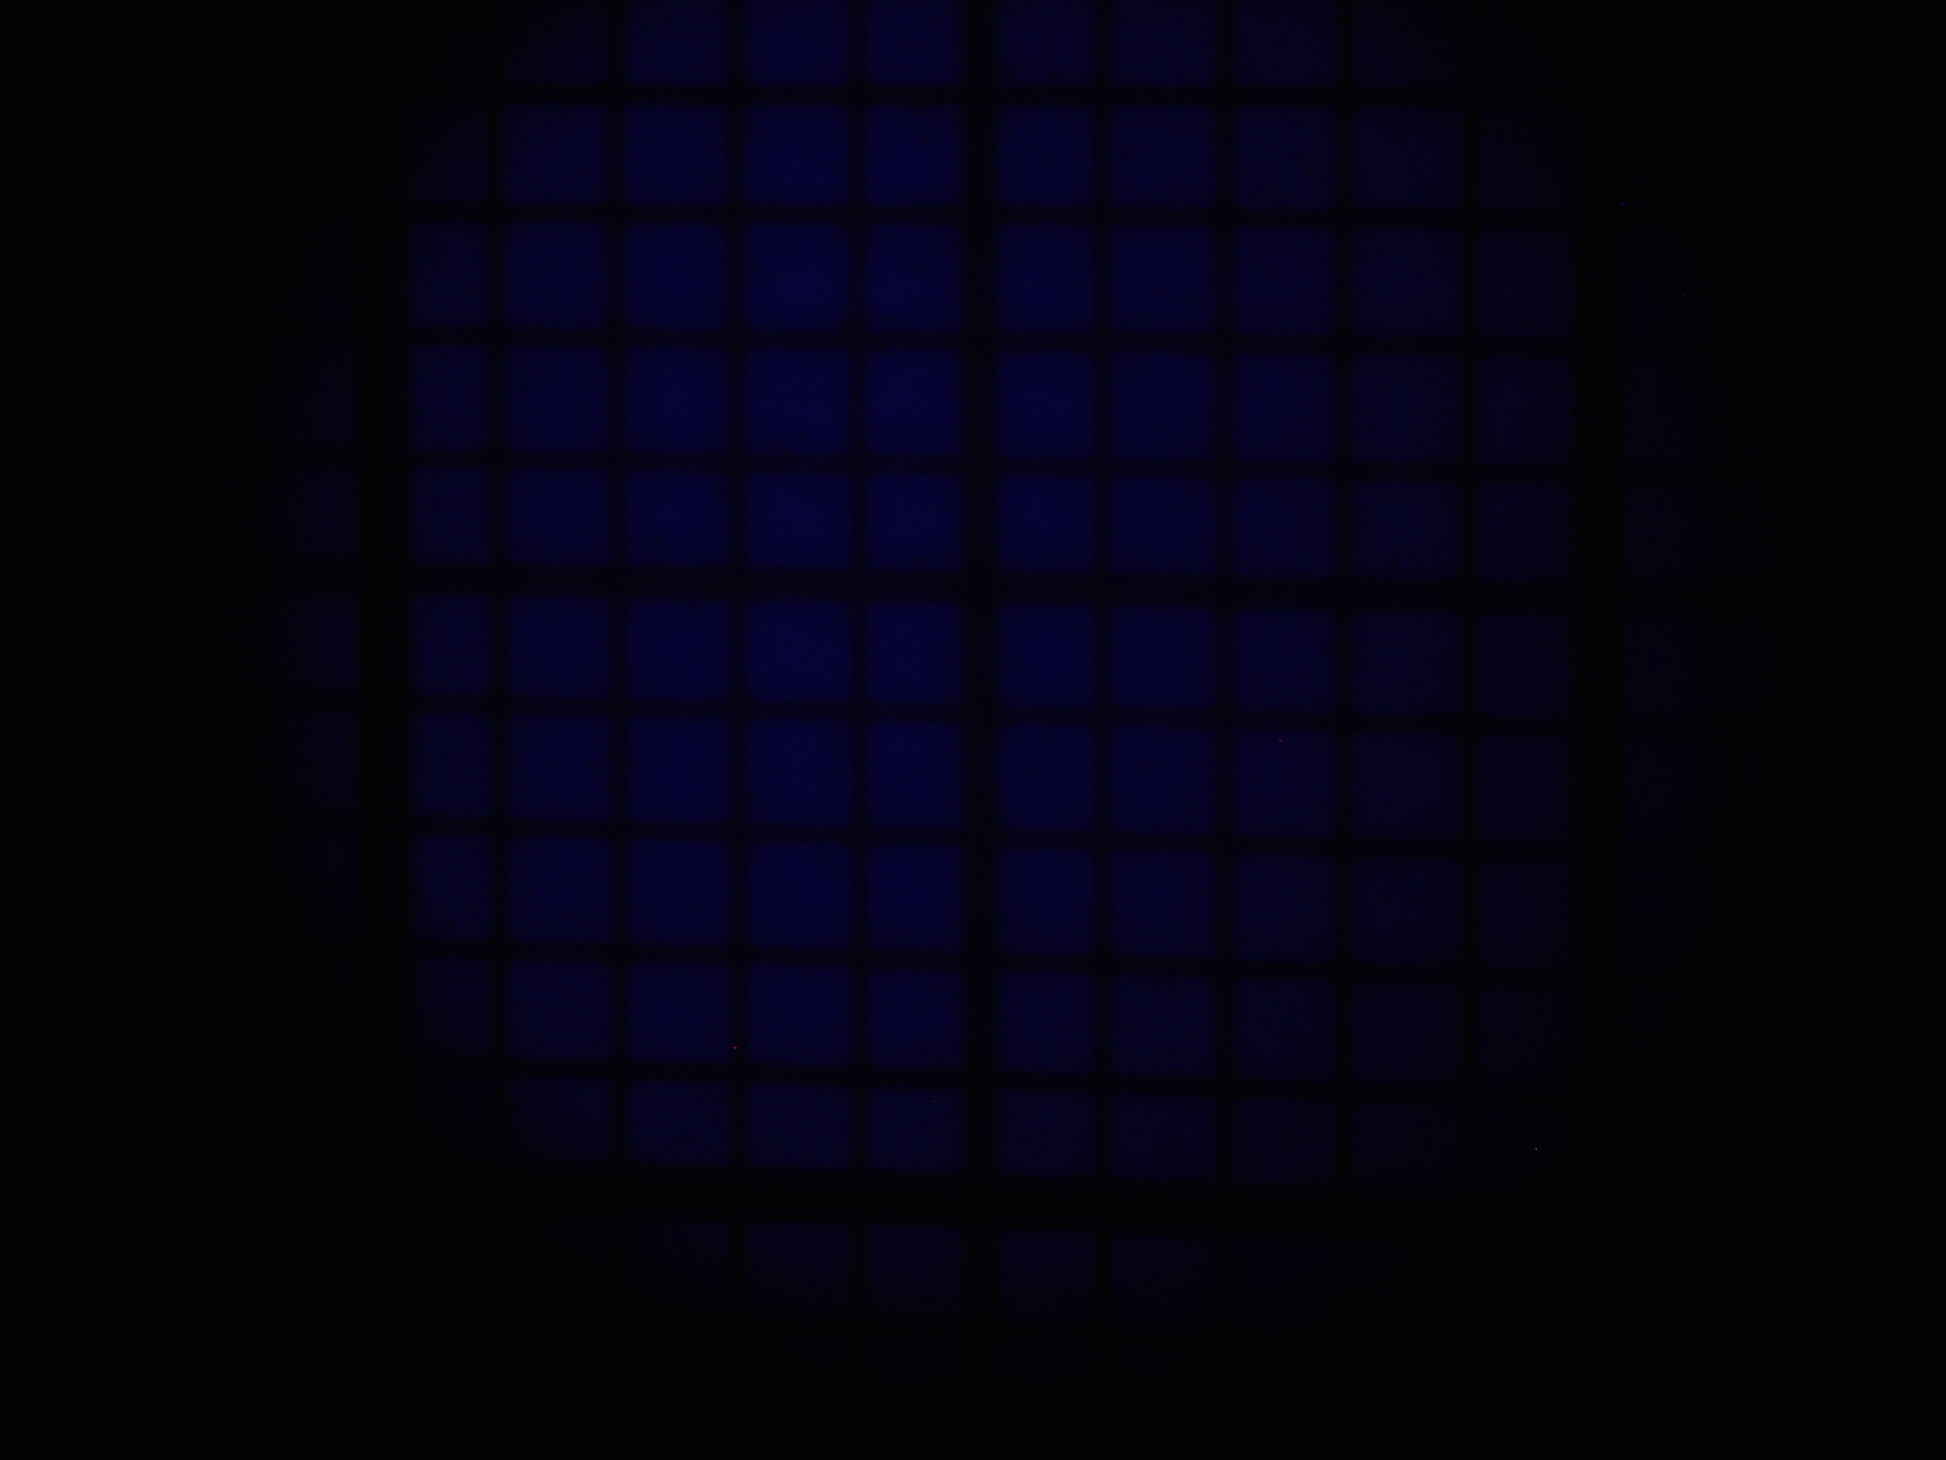
\includegraphics[clip=true, trim=700px 950px 900px 250px, width=\linewidth]{img/ChromAbb/Prakt_Linsenfehler_2015_06_04_071}
		\caption{Fokussierte Abbildung der blauen Wellenlängen (Achromat)}
		\label{fig:cm_blau_achromat}
	\end{minipage}
	\hfill
	\begin{minipage}[t]{0.32\textwidth}
		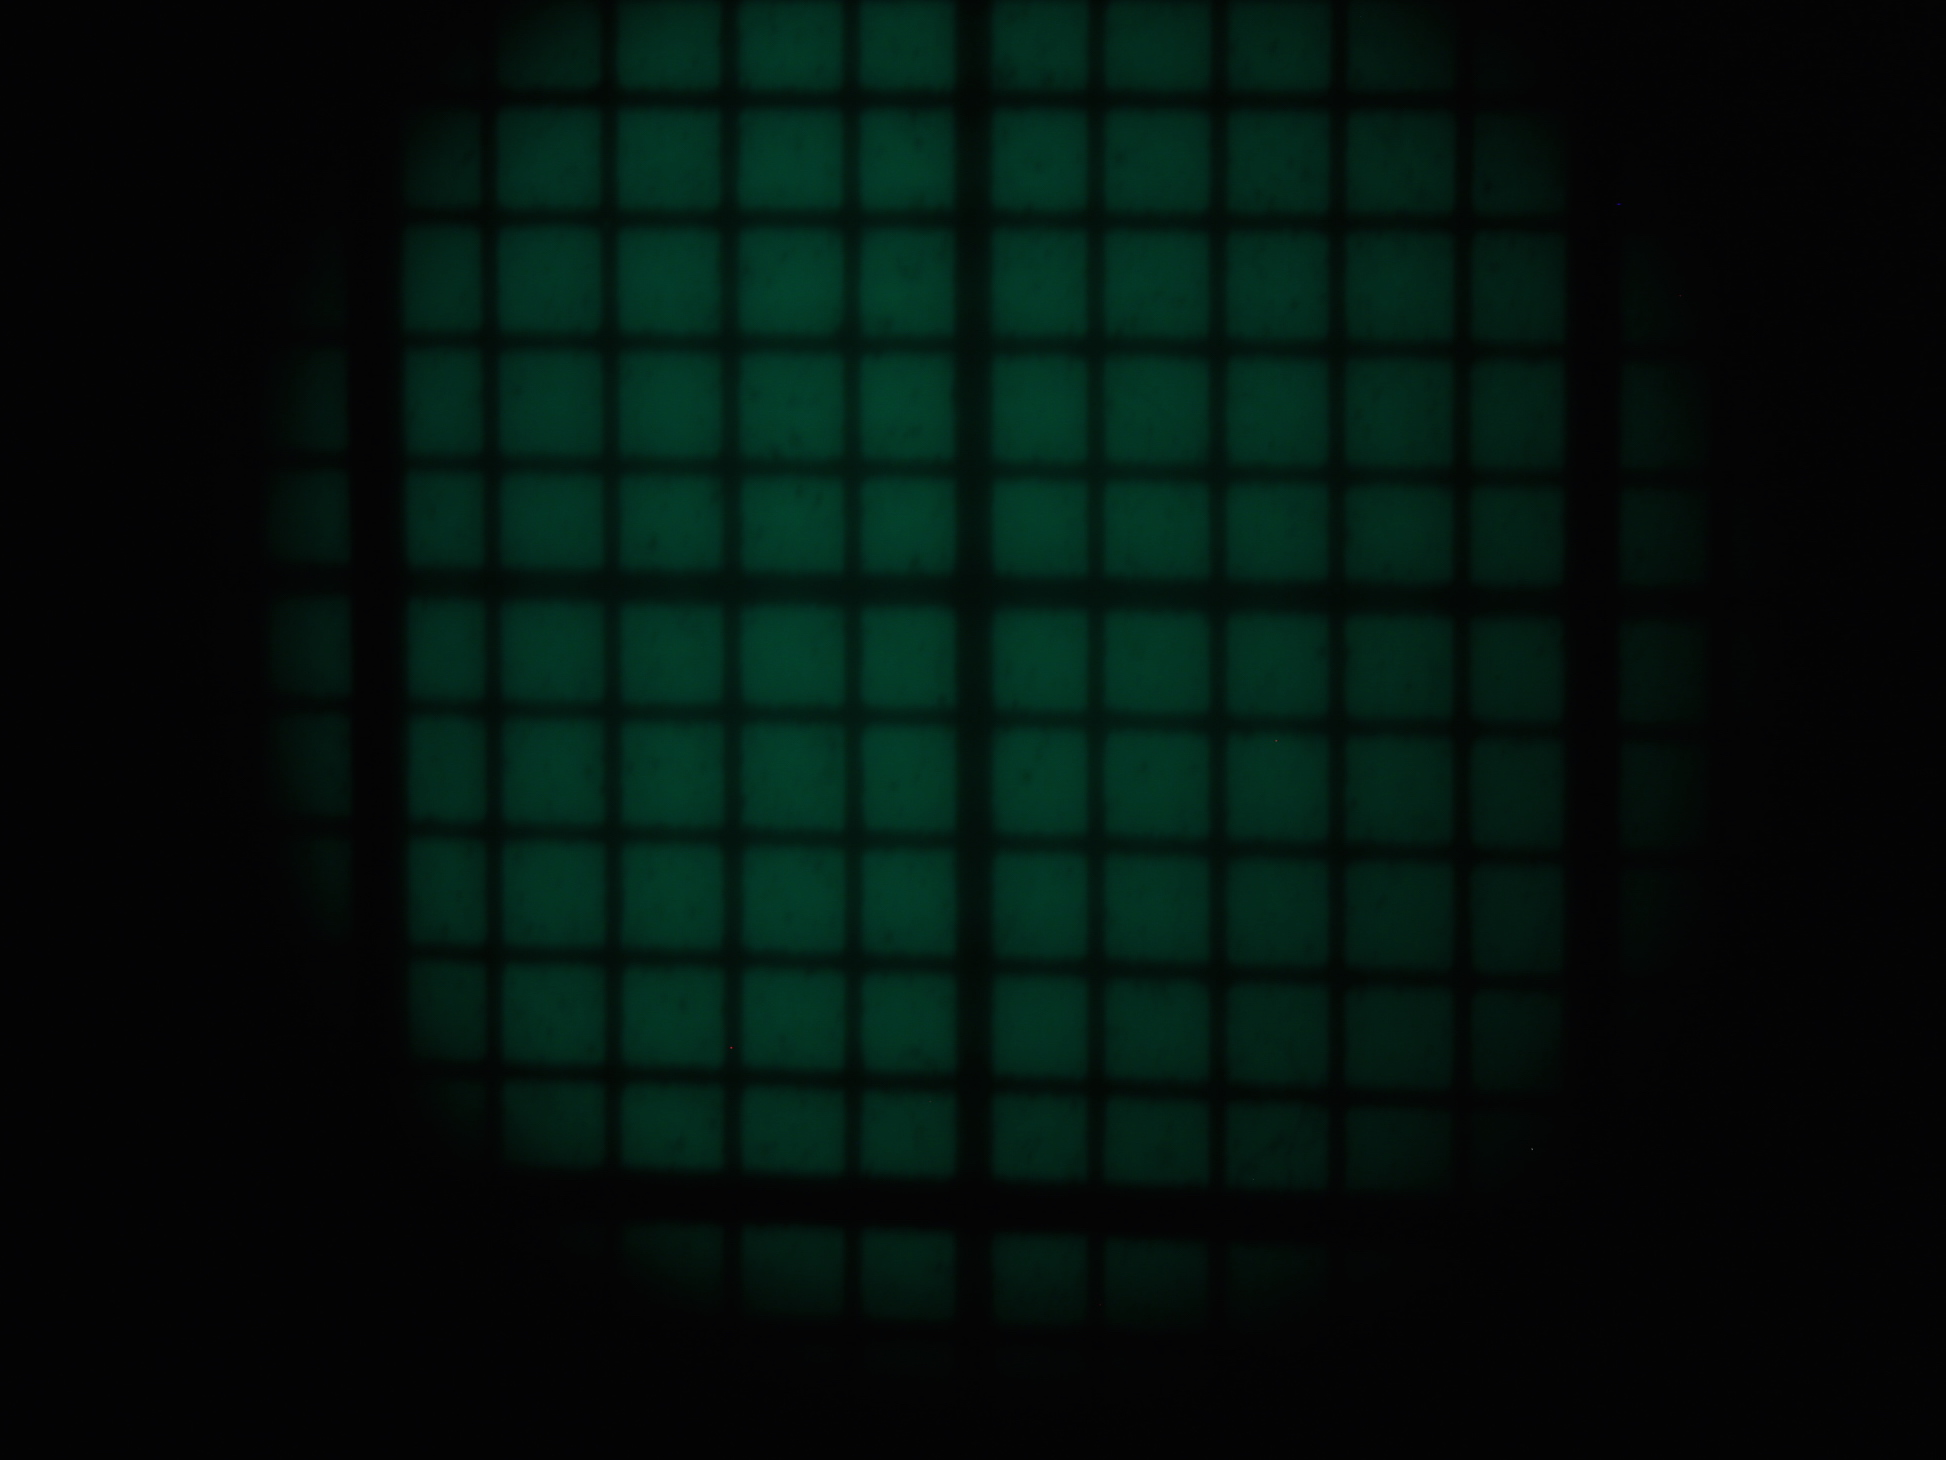
\includegraphics[clip=true, trim=700px 950px 900px 250px, width=\linewidth]{img/ChromAbb/Prakt_Linsenfehler_2015_06_04_072}
		\caption{Fokussierte Abbildung der grünen Wellenlängen (Achromat)}
		\label{fig:cm_gruen_achromat}
	\end{minipage}
	\hfill
	\begin{minipage}[t]{0.32\textwidth}
		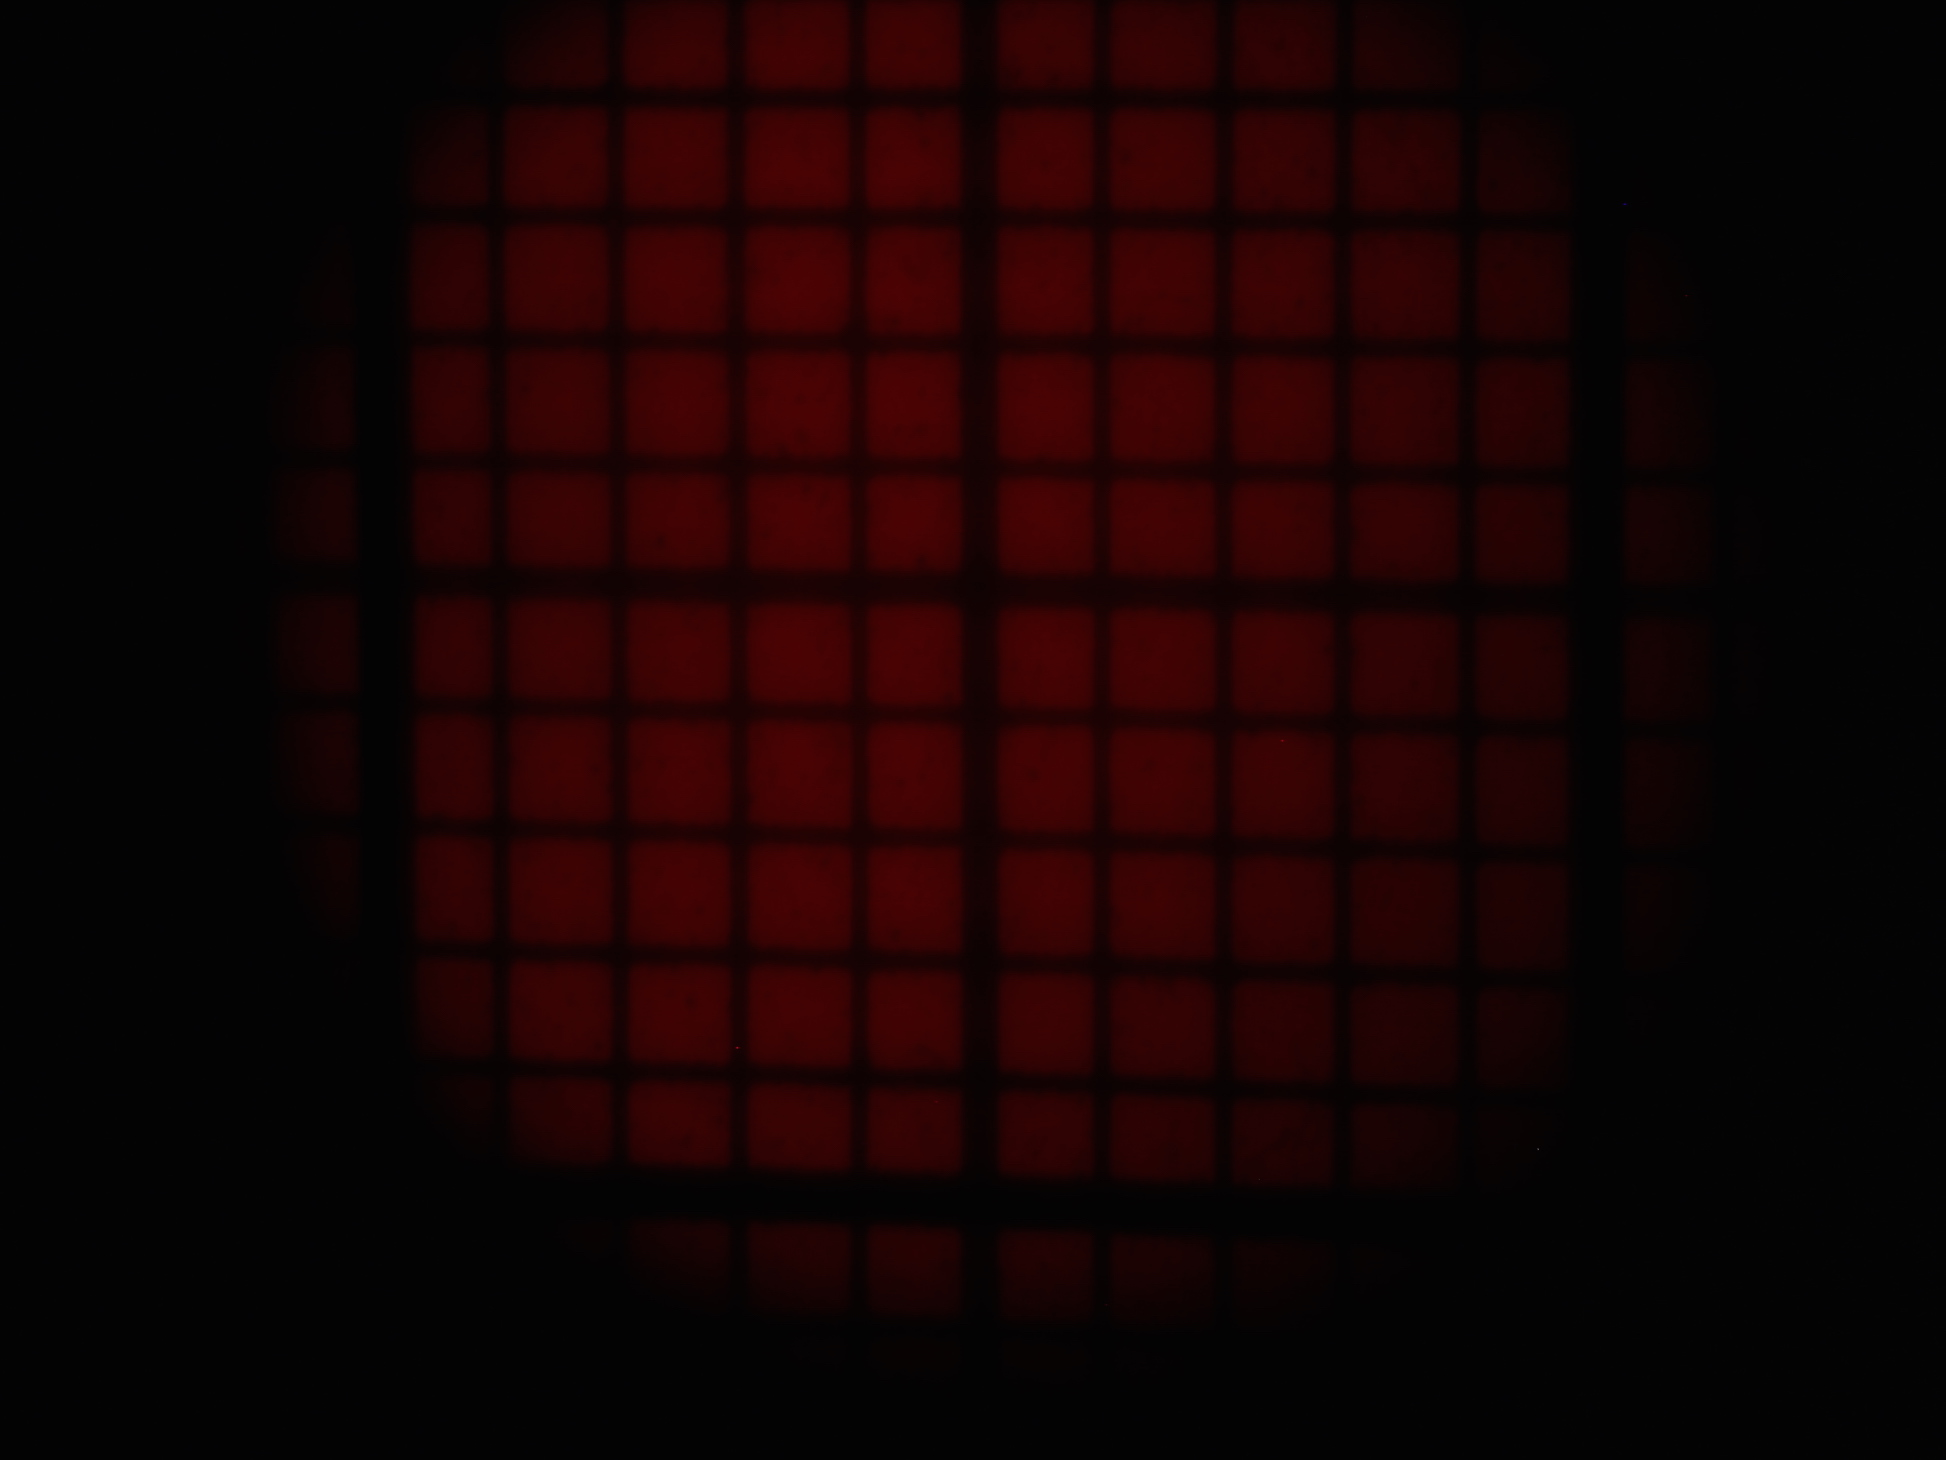
\includegraphics[clip=true, trim=700px 950px 900px 250px, width=\linewidth]{img/ChromAbb/Prakt_Linsenfehler_2015_06_04_073}
		\caption{Fokussierte Abbildung der roten Wellenlängen (Achromat)}
		\label{fig:cm_rot_achromat}
	\end{minipage}
\end{figure}


